\documentclass[12pt,a4paper]{report}
\usepackage[utf8]{inputenc}
\usepackage[T1]{fontenc}
\usepackage{geometry}
\geometry{a4paper, margin=2.5cm}
\usepackage{setspace}
\onehalfspacing
\usepackage{graphicx}
\usepackage{booktabs}
\usepackage{array}
\usepackage{longtable}
% Full-grid table style
\setlength{\arrayrulewidth}{0.4pt}
\renewcommand{\arraystretch}{1.3}
\usepackage{hyperref}
\hypersetup{colorlinks=true, linkcolor=blue, citecolor=blue, urlcolor=blue}
\usepackage{amsmath}
\usepackage{float}
\usepackage{caption}
\usepackage{subcaption}
\usepackage{fancyhdr}
\usepackage{titlesec}
\usepackage{parskip}
\usepackage{xcolor}
\usepackage{multirow}
\usepackage{listings}
\usepackage{tikz}
\usetikzlibrary{patterns, calc}

\lstset{
  basicstyle=\ttfamily\small,
  backgroundcolor=\color{gray!10},
  frame=single, breaklines=true,
  keywordstyle=\color{blue},
  commentstyle=\color{green!60!black},
  stringstyle=\color{red!70!black},
}

\graphicspath{{figures/}{run_graphs/}{run_graphs/ThermalDrone/}}

\pagestyle{fancy}
\fancyhf{}
\rhead{\small AI Multi-Agent Anti-UAV Detection System}
\lhead{\small \leftmark}
\cfoot{\thepage}

% Allow slightly loose line breaking to prevent overfull hboxes
\sloppy

\titleformat{\chapter}[display]
{\normalfont\huge\bfseries}{\chaptertitlename\ \thechapter}{20pt}{\Huge}
\titlespacing*{\chapter}{0pt}{50pt}{40pt}

\begin{document}

\begin{titlepage}
  \centering
  \vspace*{2cm}
  {\scshape\LARGE University of Khartoum \par}
  \vspace{0.4cm}
  {\scshape\large Faculty of Engineering \par}
  \vspace{0.2cm}
  {\scshape\large Department of Electrical and Electronics Engineering \par}
  \vspace{3cm}
  \rule{\linewidth}{0.5mm}\\[0.4cm]
  {\huge\bfseries AI Multi-Agent Anti-UAV Detection System\\[0.4cm]
    A Distributed Edge-Computing Framework\\[0.3cm]
    for Real-Time Anti-UAV Detection and Tracking\par}
  \rule{\linewidth}{0.5mm}\\[1.5cm]
  \vspace{1cm}
  {\Large\itshape Project Report --- Updated April 2026\par}
  \vspace{2cm}
  {\large
    \textbf{Authors:}\\[0.3cm]
    Abdelsamad Abdalla Abdelsamad\\
    Mustafa Mubarak Elsaeed\\[0.5cm]
    \textbf{Supervisor:}\\[0.3cm]
    D. Magdi Amen\\[1cm]
  }
  \vfill
  {\large April 2026\par}
\end{titlepage}

\tableofcontents
\newpage

\begin{abstract}
This report presents the complete design, implementation, and experimental
evaluation of an AI-powered distributed anti-UAV detection system. The system
combines a YOLO26s object detection model running on edge devices with a
centralised control center accessible via web browser and mobile devices.

The production model, \textbf{BirdDrone-2C-FT}, is a fine-tuned 2-class
Bird/Drone YOLO26s detector trained on curated aerial imagery and subsequently
fine-tuned on pseudo-labeled frames from the DUT Anti-UAV benchmark.
It achieves mAP@0.5 = 0.969 on the combined validation set, an average
detection rate of 0.818 across 20 DUT benchmark videos, and a bird false
alarm rate of just 0.3\%. Fine-tuning reduces low-confidence false positives
by 55\% compared to the base model, with negligible regression on original
validation sets.

A separate \textbf{ThermalDrone} model (1-class: Drone) was trained on the
SIDD thermal infrared dataset (3,788 images, 4 scenes) using thermal-specific
augmentation (HSV disabled, high copy-paste, random erasing for CCTV overlay
simulation). It achieves mAP@0.5 = 0.958 on the SIDD validation split.
Evaluated on the Anti-UAV410 thermal benchmark (129,691 frames, 128 test
sequences), it achieves Precision = 0.993, Recall = 0.730, F1 = 0.842,
and a Detection Rate of 0.730 on visible frames.

The control center provides JWT-based authentication with invite-token
registration, a real-time dashboard with per-class detection color coding,
an interactive map with slide-in device panels, WebRTC live video streaming,
and edge device health monitoring.
\end{abstract}

% ============================================================
\chapter{Introduction}

\section{Background of the Study}

In recent years, electrical and computer engineering systems have experienced
significant technological advancements, particularly in the areas of artificial
intelligence, computer vision, and distributed embedded computing. Unmanned
aerial vehicles (UAVs), commonly known as drones, have proliferated rapidly
across both consumer and commercial markets. Originally confined to military
applications, UAVs are now widely used in photography, agriculture, logistics,
and infrastructure inspection.

This technological democratisation has, however, introduced serious security
challenges. Consumer drones are increasingly exploited for surveillance,
smuggling, and attacks on critical infrastructure. Airports, power stations,
government facilities, and public events are all vulnerable to unauthorised
UAV incursions. Vision-based anti-UAV detection systems have emerged as a
cost-effective countermeasure, leveraging advances in deep learning object
detection to identify and track aerial threats in real time.

A key challenge in vision-based UAV detection is the visual similarity
between drones and birds at long range. Both occupy the same low-altitude
airspace, exhibit similar apparent sizes at distance, and move in comparable
flight patterns. Distinguishing between them is the central technical problem
that this project addresses.

\section{Problem Statement}

Existing anti-UAV detection systems suffer from three principal limitations.
First, single-class drone detectors do not distinguish between drones and
birds, leading to high false alarm rates in environments with bird activity.
Second, models trained on clean benchmark datasets degrade significantly
when deployed on real-world sequences with complex backgrounds such as
urban structures, tree canopies, and sky gradients. Third, most published
systems operate as standalone detectors without a distributed architecture
that allows multiple edge nodes to be monitored and controlled from a
centralised interface.

These limitations reduce the operational utility of existing systems:
a detector that generates frequent false alarms on birds will be disabled
by operators, and a system that cannot be monitored centrally cannot be
deployed at scale across a protected perimeter.

\section{Significance of the Project}

This project contributes to the field of airspace security and intelligent
embedded systems in the following ways:

\begin{itemize}
  \item \textbf{Academic contribution}: Demonstrates a complete pipeline
        from dataset curation and model training to real-world evaluation
        on the DUT Anti-UAV benchmark, providing reproducible baselines
        for the Bird/Drone discrimination task.
  \item \textbf{Practical contribution}: Delivers a deployable distributed
        detection system with a web-based control center, enabling real-time
        monitoring of multiple edge nodes from a single interface.
  \item \textbf{Technical contribution}: Introduces a pseudo-label fine-tuning
        methodology that improves detection continuity on real-world sequences
        without requiring manual annotation of the fine-tuning data.
\end{itemize}

\section{Project Objectives}

The general objective of this project is to design, implement, and evaluate
an AI-powered distributed anti-UAV detection system capable of real-time
bird/drone discrimination on edge hardware with centralised web-based monitoring.

The specific objectives are:

\begin{enumerate}
  \item Design and implement a 2-class aerial object detection model (Bird, Drone)
        using YOLO26s, trained on curated RGB datasets with balanced class representation.
  \item Design and implement a pseudo-label fine-tuning pipeline on the DUT Anti-UAV
        benchmark to improve real-world detection continuity and reduce false positives.
  \item Implement a distributed edge-computing inference pipeline with
        MQTT communication, WebRTC live streaming, and PTZ camera control.
  \item Design and implement a web-based control center with JWT authentication,
        real-time monitoring, and multi-device management.
  \item Train and evaluate a dedicated thermal infrared detection model
        (ThermalDrone) on the SIDD dataset and benchmark it against the
        Anti-UAV410 thermal infrared benchmark to establish a thermal
        detection baseline for 24/7 operation.
\end{enumerate}

\section{Scope and Limitations}

\begin{itemize}
  \item Training datasets are limited to publicly available RGB drone and
        bird imagery (CC BY 4.0 and CC0 licenses).
  \item Thermal infrared modality is partially addressed: a 1-class
        ThermalDrone model has been trained on the SIDD thermal dataset
        and evaluated on the Anti-UAV410 benchmark
        (Section~\ref{sec:thermal_results}). Full 24/7 thermal deployment
        requires additional dataset acquisition.
  \item The DUT Anti-UAV evaluation uses proxy metrics (detection rate,
        tracking gaps) since per-frame annotations are not available in
        the tracking split.
  \item The system is evaluated under normal lighting and weather conditions;
        adverse weather robustness is not assessed in the current work.
\end{itemize}

The thermal infrared gap deserves specific mention. Delleji et al.~\cite{delleji2025thermal}
demonstrate that existing public thermal datasets are inadequate for aerial
drone detection: the FLIR ADAS dataset targets automotive scenes, the KAIST
Multispectral dataset focuses on pedestrian detection, and available aerial
thermal datasets contain fewer than 2,000 frames with minimal diversity.
Their work further shows that a custom thermal pipeline --- capturing three
DJI UAV types at multiple altitudes with a 640$\times$512 LWIR sensor ---
is necessary to achieve reliable thermal detection. This confirms that
extending BirdDrone-2C-FT to the thermal modality requires a dedicated
dataset acquisition effort beyond the scope of the current work.

\section{Methodology Overview}

The methodology follows four main stages: dataset curation and preparation,
model training and fine-tuning, system implementation, and performance
evaluation. Full implementation details are provided in Chapter~3.

\section{Report Structure}

Chapter~2 provides the theoretical background and literature review.
Chapter~3 describes the full methodology including requirements, system
framework, datasets, and implementation. Chapter~4 presents training and
evaluation results. Chapter~5 discusses the findings. Chapter~6 concludes
with deployment recommendations and future work.

% ============================================================
\chapter{Literature Review}

\section*{Part I: Theoretical Background}
\addcontentsline{toc}{section}{Part I: Theoretical Background}

\section{Fundamental Concepts}

\subsection{Object Detection and the YOLO Paradigm}

Object detection is the computer vision task of simultaneously localising
and classifying all objects of interest within an image. A detector outputs
a set of bounding boxes, each described by its centre coordinates $(x, y)$,
width $w$, height $h$, a class label, and a confidence score $p$.

Single-stage detectors such as YOLO (You Only Look Once) perform detection
in a single forward pass through a convolutional neural network, making them
suitable for real-time applications. The network divides the input image into
a grid and predicts bounding boxes and class probabilities directly from each
grid cell. The key performance metric is mean Average Precision (mAP), defined
as the area under the precision-recall curve averaged over all classes and
IoU thresholds.

\subsection{Transfer Learning}

Transfer learning is the practice of initialising a model with weights
pre-trained on a large dataset (e.g., COCO) and then fine-tuning it on a
smaller domain-specific dataset. This approach is standard in aerial object
detection because domain-specific datasets are typically small relative to
the number of model parameters. The pre-trained backbone learns general
visual features (edges, textures, shapes) that transfer well to new domains,
while the detection head is adapted to the target class set.

\subsection{Edge Computing for Real-Time Inference}

Edge computing refers to the deployment of computation close to the data
source, rather than in a centralised cloud. For UAV detection, edge
deployment means running the YOLO inference engine on a device co-located
with the camera (e.g., Raspberry Pi 4, NVIDIA Jetson Nano), reducing
network latency and enabling operation in environments without reliable
internet connectivity. The trade-off is limited computational resources:
edge devices have constrained VRAM, CPU/GPU performance, and power budgets.

\subsection{MQTT and Publish-Subscribe Communication}

MQTT (Message Queuing Telemetry Transport) is a lightweight publish-subscribe
messaging protocol designed for constrained devices and low-bandwidth networks.
In the proposed system, each edge node publishes detection results to an MQTT
broker; the control center subscribes to these topics and aggregates the
results in real time. MQTT's low overhead makes it suitable for transmitting
frequent detection messages (up to 25 per second per node) without saturating
the network.

\subsection{WebRTC for Live Video Streaming}

WebRTC (Web Real-Time Communication) is an open standard for peer-to-peer
audio and video communication directly in web browsers. It enables low-latency
live video streaming from edge cameras to the control center without requiring
a dedicated media server. The control center uses WebRTC to display live
camera feeds alongside detection overlays.

\section{Related Systems and Models}

\subsection{Distributed Anti-UAV Detection Architectures}

A distributed anti-UAV system consists of multiple sensor nodes (cameras,
radars, or acoustic sensors) connected to a central command and control
system. Vision-based distributed systems use cameras at each node, running
local inference to reduce bandwidth requirements. The central system
aggregates detections, maintains a common operational picture, and allows
operators to task individual nodes (e.g., PTZ camera control).

The two-tier architecture adopted in this project --- edge inference nodes
communicating over MQTT to a web-based control center --- is consistent
with the distributed paradigm described in the literature. Each tier has
distinct responsibilities: the edge tier handles computationally intensive
inference, while the control tier handles aggregation, visualisation, and
operator interaction.

\subsection{YOLO-Based Aerial Object Detectors}

The YOLO family has been the dominant architecture for aerial object
detection since YOLOv3. Key variants relevant to this work include:
YOLOv5 (used in the KFUPM anti-UAV system), YOLOv8 (used in the
Drone-vs-Bird challenge), and YOLO26 (used in this project). Each
successive version improves small-object detection through architectural
changes to the feature pyramid network and label assignment strategy.

\section{Techniques, Methods, and Algorithms}

\subsection{Pseudo-Label Fine-Tuning}

Pseudo-labeling is a semi-supervised learning technique in which a trained
model generates labels for unlabeled data, and these generated labels are
used as training targets for a subsequent fine-tuning stage. In this project,
the base BirdDrone-2C model generates bounding box annotations for frames
in the DUT Anti-UAV tracking split (which lacks per-frame ground-truth
annotations). Only frames where the model's confidence exceeds 0.70 are
retained, ensuring label quality. The fine-tuned model is then trained on
the combination of the original labeled data and the pseudo-labeled DUT frames.

\subsection{Data Augmentation for Aerial Detection}

Data augmentation artificially increases training set diversity by applying
geometric and photometric transformations to existing images. For aerial
object detection, the most effective augmentations are:
\begin{itemize}
  \item \textbf{Copy-paste}: Pastes object crops onto diverse backgrounds,
        directly increasing background variety for small aerial targets.
  \item \textbf{Rotation}: Simulates drones at arbitrary orientations.
  \item \textbf{Vertical flip}: Simulates upward-facing camera perspectives.
  \item \textbf{Mosaic}: Combines four images into one, increasing object
        density and scale variety per training step.
\end{itemize}

\subsection{ByteTrack Multi-Object Tracking}

ByteTrack is a multi-object tracking algorithm that associates detections
across frames using the Hungarian algorithm with IoU-based cost matrices.
Unlike trackers that discard low-confidence detections, ByteTrack retains
them as secondary candidates, improving tracking continuity when the detector
is momentarily uncertain. This is particularly valuable for small aerial
targets that may produce low-confidence detections at long range.

\section*{Part II: Literature Review}
\addcontentsline{toc}{section}{Part II: Literature Review}

\section{YOLO Model Family}

The YOLO (You Only Look Once) family of single-stage object detectors has
dominated real-time detection benchmarks since its introduction. YOLO26~\cite{ultralytics2025},
released by Ultralytics in September 2025, introduces several key innovations
relevant to aerial UAV detection:

\begin{itemize}
  \item \textbf{NMS-free end-to-end inference}: eliminates non-maximum
        suppression post-processing, reducing deployment latency.
  \item \textbf{MuSGD optimizer}: momentum-updated SGD with improved
        convergence on small and imbalanced datasets.
  \item \textbf{STAL (Small-Target-Aware Label Assignment)}: improves
        detection of small objects, directly addressing distant drones.
  \item \textbf{DFL removal}: simplified distribution focal loss reduces
        model complexity without sacrificing accuracy.
\end{itemize}

YOLO26s (9.9M parameters, 22.5 GFLOPs) was selected for this work as it
fits within the RTX 2070 8GB VRAM budget at batch 16 (4.7GB peak) while
providing state-of-the-art accuracy for aerial imagery. The ``s'' (small)
variant is also deployable on edge hardware such as Raspberry Pi 4 and
NVIDIA Jetson Nano, making it suitable for the distributed inference
architecture of this system.

\section{Drone vs.\ Bird Detection}

The Drone-vs-Bird Detection Grand Challenge (WOSDETC)~\cite{coluccia2023},
held annually at AVSS, ICIAP, and ICASSP, provides the most directly
comparable benchmark. The 2023 edition reported top methods achieving
F1 $\approx$ 0.91 (OBSS, 1st place) and 0.88 (multi-scale YOLOv8,
IJCNN 2025)~\cite{simd3_2025}. The challenge uses RGB video sequences
with small drone targets against complex backgrounds including birds.

YOLOBirDrone~\cite{yolobirdrone2025} (arXiv:2601.08319) proposes a
dedicated dataset and enhanced YOLO architecture for bird vs.\ drone
classification, reporting improved discrimination over standard YOLO
baselines. Their work confirms that the Bird/Drone boundary is the
primary challenge in aerial detection systems --- the same challenge
that BirdDrone-2C-FT is specifically designed to address.

\section{UAV Detection Under Adverse Conditions}

Real-world anti-UAV systems must operate in conditions that deviate
significantly from the clean, well-lit imagery used in most benchmark
evaluations. Munir~\cite{munir2023kfupm} provides the first systematic
study of UAV detection under adverse weather, introducing three
weather-affected test sets derived from the Anti-UAV dataset: RTD
(drizzle, heavy, and torrential rain), ANTD (low, medium, and high
additive white Gaussian noise), and MBTD (low, medium, and high motion
blur). The results are striking: YOLOv5m, the strongest baseline on
clean data (mAP@0.5 = 95.6\%), degrades to 47.9\% under torrential rain
and 21.9\% under high motion blur --- performance drops of 50.6 and
77.0 percentage points respectively.

To address this, Munir proposes YOLO-RAW, a multi-scale UAV detector
that extends YOLOv5 with: an additional CBS+C3 block in the CSPDarknet53
backbone, an SPPF-Enhanced module, four SimAM (Simple, Parameter-Free
Attention Module) blocks in the neck, and a fourth prediction head (P6)
for large-scale objects via PANet extension. YOLO-RAW achieves 95.2\%
mAP@0.5 on the Complex Background Dataset and outperforms YOLOv5m on
all weather-affected test sets. Critically, training with weather-augmented
data (33\% noisy + 33\% motion-blurred + 34\% rainy images) improves
YOLOv5m's torrential rain performance from 47.9\% to 83.3\% mAP@0.5
and high-blur performance from 21.9\% to 66.8\%, while clean-data
mAP@0.5 drops only marginally from 95.6\% to 94.6\%. This demonstrates
that weather augmentation is a low-cost, high-impact robustness strategy
directly applicable to YOLO26s training.

\section{Transfer Learning for Aerial Object Detection}

Transfer learning from large-scale detection models to domain-specific
aerial datasets has emerged as the dominant training paradigm for UAV
detection. Reis et al.~\cite{reis2024yolov8} demonstrate a two-stage
transfer learning strategy: a generalised YOLOv8 model is first trained
on 15,064 images across 40 flying object classes (mAP@0.5 = 79.2\%,
mAP@0.5:0.95 = 68.5\%, 50 fps on 1080p), then transfer-learned to a
3-class refined model (drone, plane, helicopter) achieving mAP@0.5 = 99.1\%,
mAP@0.5:0.95 = 83.5\%, at 50 fps. The two-stage approach --- learning
abstract flying-object features first, then specialising to a narrow
class set --- is directly analogous to the BirdDrone-2C base training
followed by DUT fine-tuning described in this report.

Reis et al.\ also provide a comparative analysis of model sizes: small
(11.1M parameters), medium (25.9M), and large (43.7M) YOLOv8 variants.
The jump in mAP@0.5:0.95 from small to medium is 0.05, but only 0.002
from medium to large, confirming diminishing returns at larger model
sizes. This analysis supports the selection of YOLO26s (9.9M parameters)
as the deployment model: it occupies the small-model tier while benefiting
from YOLO26's architectural improvements (STAL, NMS-free inference) that
were not available to the YOLOv8 small variant.

\section{DUT Anti-UAV Benchmark}

The DUT Anti-UAV dataset~\cite{dutantiuav2022} (IEEE-TITS 2022) provides
20 RGB daytime UAV detection sequences with published baselines:
YOLOX 0.720, Cascade-RCNN 0.680, ATSS 0.665, Faster R-CNN 0.621.
The dataset is particularly challenging due to complex backgrounds
(buildings, trees, sky) and small UAV apparent sizes at distance.
BirdDrone-2C-FT achieves an average detection rate of 0.818 on these
sequences, exceeding the published YOLOX baseline.

\section{Transfer Learning and Fine-Tuning for Aerial Detection}

Transfer learning from large-scale detection models to domain-specific
aerial datasets is well-established. The key challenge is catastrophic
forgetting: aggressive fine-tuning can erase generalisation learned during
base training. This work addresses this by using a 10$\times$ reduced
learning rate (lr0 = 0.001 vs 0.01 for base training), short patience
(8 epochs), and copy-paste augmentation to maintain diversity in the
fine-tuning data.

\section{Data Quality in Aerial Detection Datasets}

A recurring finding in aerial detection research is that dataset quality
matters more than dataset size. Delleji et al.~\cite{delleji2025thermal}
validate this principle experimentally in the thermal domain: after
cleaning a 12,600-image thermal dataset down to 10,200 images using
perceptual hashing (phash, hash size 8, Hamming distance threshold),
YOLOv11 precision and recall remained equivalent or improved. Removing
near-duplicates, mislabeled samples, and low-quality frames had no
negative impact on model performance --- a result the authors summarise
as ``good data beats more data.''

This principle directly informs the dataset curation strategy for
BirdDrone-2C. Rather than using all 19,849 available drone images from
the anti-uav Roboflow dataset, the training set was capped at 2,850
images to maintain 50/50 class balance with the 3,404 bird images.
The deliberate choice to prioritise balance and quality over raw volume
is consistent with the findings of Delleji et al.\ and with the
pseudo-labeling confidence threshold of 0.70 applied during DUT
fine-tuning, which excludes uncertain frames rather than accepting
all available annotations.

\section{Distributed Edge Inference}

Stacker et al.~\cite{stacker2021} (ICCVW 2021) demonstrate that runtime
optimisation techniques (quantisation, TensorRT export, batch size tuning)
are critical for achieving acceptable inference throughput on resource-constrained
edge hardware. This informs our model selection (YOLO26s over larger variants)
and configurable frame rate design.

Stäcker et al.\ provide quantitative benchmarks on NVIDIA Jetson AGX Xavier
that are directly applicable to this system's edge deployment targets.
Using TensorRT with Int8 quantisation and entropy calibration, RetinaNet-18
inference time drops from 104 ms (Float32) to 25 ms --- a 4.2$\times$
speedup with minimal accuracy loss (mAP: 0.361 $\to$ 0.355). Float16
quantisation achieves 38 ms with near-identical accuracy (mAP: 0.356),
making it the preferred option when calibration data is unavailable.
Notably, input resolution has a larger impact on detection performance
than quantisation format: mAP increases from 0.298 (low resolution,
416$\times$736) to 0.393 (high resolution, 832$\times$1472) with Int8,
suggesting that maintaining adequate input resolution is more important
than precision format on constrained hardware.

Power supply mode introduces a further constraint: on Jetson AGX Xavier,
reducing power from 50W (MAXN) to 10W increases the full detection
pipeline latency from 31 ms to 107 ms --- a 3.5$\times$ slowdown for
a 5$\times$ power reduction. For battery-powered or solar-powered
distributed anti-UAV nodes, this trade-off must be explicitly managed
through power budget planning. The Deployment Recommendations in
Chapter~6 reflect these findings by recommending TensorRT INT8 export
for resource-constrained edge hardware.

\section{Distance and Trajectory Estimation}

When enabled, the system estimates UAV distance using the pinhole camera model:

\begin{equation}
d = \frac{W_{\text{real}} \cdot f}{W_{\text{bbox}}}
\quad \text{where} \quad
f = \frac{W_{\text{frame}}}{2 \tan(\theta_{\text{FOV}}/2)}
\end{equation}

where $W_{\text{real}}$ is the known UAV wingspan (configurable, default 0.5m),
$W_{\text{bbox}}$ is the bounding box width in pixels, and $\theta_{\text{FOV}}$
is the camera horizontal field of view. Trajectory estimation computes the
mean frame-to-frame centroid displacement over a rolling window of $N$ frames.

\section{Comparative Analysis of Previous Work}

Table~\ref{tab:lit_compare} summarises the key prior systems reviewed in
this chapter, comparing their detection approach, dataset, and reported
performance.

\begin{table}[H]
\centering
\caption{Comparative analysis of related anti-UAV detection systems.}
\label{tab:lit_compare}
\small
\begin{tabular}{|p{3.0cm}|p{2.4cm}|p{2.4cm}|p{2.4cm}|p{2.4cm}|}
\hline
\textbf{Work} & \textbf{Model} & \textbf{Dataset} & \textbf{Performance} & \textbf{Limitation} \\
\hline
Munir~\cite{munir2023kfupm} (2023) & YOLO-RAW (YOLOv5 extension) & Anti-UAV + weather-augmented & 95.2\% mAP@0.5 (clean) & Single-class; no bird discrimination \\
\hline
Coluccia et al.~\cite{coluccia2021sensors} (2021) & Various (challenge) & DvB Grand Challenge & F1 up to 0.91 & No distributed deployment \\
\hline
Reis et al.~\cite{reis2024yolov8} (2024) & YOLOv8 (multi-size) & 15,064 flying objects & 99.1\% mAP@0.5 (3-class) & No bird class; no edge deployment \\
\hline
Stäcker et al.~\cite{stacker2021} (2021) & RetinaNet-18 (TensorRT) & COCO + custom & 0.361 mAP (Int8) & Detection only; no control center \\
\hline
Delleji et al.~\cite{delleji2025thermal} (2025) & YOLOv11 & Custom thermal & High precision/recall & Thermal only; no RGB \\
\hline
\textbf{This work (RGB)} & \textbf{YOLO26s (BirdDrone-2C-FT)} & \textbf{BirdDrone-2C + DUT} & \textbf{0.969 mAP@0.5} & \textbf{RGB only; no weather eval} \\
\hline
\textbf{This work (Thermal)} & \textbf{YOLO26s (ThermalDrone)} & \textbf{SIDD thermal} & \textbf{0.958 mAP@0.5 (val); F1=0.842 (Anti-UAV410)} & \textbf{1-class; SIDD training only} \\
\hline
\end{tabular}
\end{table}

The comparative analysis reveals that existing systems address either the
detection accuracy problem (Munir, Reis et al.) or the edge deployment
problem (Stäcker et al.) but not both simultaneously. None of the reviewed
systems provide a complete distributed architecture with a web-based control
center and explicit bird/drone discrimination.

\section{Multi-Object Tracking for Aerial Surveillance}

Accurate multi-object tracking is essential for maintaining persistent
identity across frames in a UAV detection system. The ByteTrack
algorithm~\cite{zhang2022bytetrack} addresses a fundamental weakness of
prior trackers: the discarding of low-confidence detections. ByteTrack
retains all detections --- including those below the confidence threshold
--- as secondary candidates and associates them with existing tracks using
IoU-based cost matrices and the Hungarian algorithm. This approach
significantly reduces identity switches and tracking gaps compared to
methods that discard uncertain detections entirely.

A comparative evaluation of ByteTrack, DeepSORT, and StrongSORT on
UAV-based video surveillance~\cite{bytetrack_comparison} demonstrates
that ByteTrack achieves the best balance of tracking accuracy and
computational efficiency for aerial surveillance applications. DeepSORT
relies on a deep appearance model (re-identification network) that adds
significant computational overhead unsuitable for edge deployment.
StrongSORT improves on DeepSORT with enhanced appearance features but
similarly requires more computation than ByteTrack. For the distributed
anti-UAV system, ByteTrack's lightweight design and superior handling of
low-confidence detections make it the preferred tracking algorithm,
particularly for small aerial targets that frequently produce uncertain
detections at long range.

\section{UAS Threat Landscape and Defense Frameworks}

The threat posed by unmanned aerial systems (UAS) to critical infrastructure
and public safety has been extensively documented. Wallace and
Loffi~\cite{wallace2015uas} provide a comprehensive conceptual analysis
of UAS threats and defenses, cataloguing seven categories of illicit UAS
use: nuisance, surveillance/reconnaissance, airspace interference,
kinetic/kamikaze attacks, payload/smuggling, weaponized platforms, and
electronic attack. Real-world incidents documented in their analysis include
a foiled 2011 FBI plot involving RC aircraft packed with explosives targeting
the Pentagon, and a hexicopter carrying methamphetamines intercepted near
the US--Mexico border in 2015.

The paper synthesises 39 unique UAS defense concepts into a five-layer
``Defense in Depth'' model: Prevention, Deterrence, Denial, Detection, and
Interruption/Destruction. Automated visual detection occupies the critical
Detection layer that enables all subsequent active responses. Miasnikov~\cite{miasnikov2005uav}
further establishes that conventional radar systems and surface-to-air
missiles are poorly suited to detecting small, slow, low-altitude
propeller-driven UAVs due to their small radar cross-sections and the
clutter-filtering algorithms that discard slow-moving objects. This gap
in traditional air defense directly motivates the need for dedicated
vision-based detection systems such as the one described in this report.

\section{Edge Computing for Distributed IoT Systems}

The deployment of AI inference on distributed edge nodes is a well-established
paradigm in the IoT literature. Kong et al.~\cite{kong2022edge} survey
edge-computing-driven IoT architectures and establish that cloud-based
processing introduces three critical bottlenecks for real-time applications:
long-haul network latency, bandwidth saturation from concurrent data streams,
and privacy risks from transmitting sensitive sensor data to remote servers.
The three-layer ECDriven-IoT architecture (endpoint devices $\to$ edge nodes
$\to$ cloud) maps directly onto the anti-UAV system's architecture: camera
nodes (endpoints) $\to$ Raspberry Pi/Jetson edge nodes $\to$ central control
server.

The survey identifies computation offloading and workload allocation as
primary design challenges: if IoT devices offload all computation to edge
servers, communication cost and edge node capacity become bottlenecks; if
devices process locally, power consumption increases. For the anti-UAV
system, this trade-off is resolved by running YOLO26s inference entirely
on the edge node (eliminating network latency for detection) while
offloading aggregation, visualisation, and storage to the central control
server.

\section{WebRTC for Real-Time Video Streaming}

WebRTC (Web Real-Time Communication) is the streaming protocol used in
this system for live camera feeds from edge nodes to the control center.
Mahmoud and Abozariba~\cite{mahmoud2025webrtc} conduct a systematic review
of 83 WebRTC studies and establish that WebRTC's peer-to-peer architecture
--- using SRTP for media encryption and DTLS for data channel security ---
eliminates the need for an intermediary media relay server in most
deployments, enabling sub-second latency streaming with mandatory
end-to-end encryption.

The review identifies NAT traversal and network congestion as the primary
reliability challenges for WebRTC in distributed deployments. STUN/TURN/ICE
solutions mitigate but do not eliminate these issues under high network
congestion. For the anti-UAV system, edge nodes behind NAT on a private
LAN require a TURN relay server as fallback, adding latency and
infrastructure cost. The signaling server in the proposed architecture
handles SDP offer/answer and ICE candidate exchange, while video flows
directly peer-to-peer between the edge device and the browser client.

\section{Vision-Based Drone Detection: Survey of Methods and Benchmarks}

Liu et al.~\cite{liu2024survey} provide a comprehensive survey of
vision-based drone detection methods in complex environments, organising
the field around four systematic challenge categories: (1) data acquisition
difficulties (limited labeled data, class imbalance), (2) background and
drone characteristics (small size, motion blur, varying drone types),
(3) imaging environment factors (weather, lighting, sensor modality), and
(4) algorithm efficiency constraints (real-time requirements, edge hardware).
This taxonomy directly maps onto the design challenges addressed in this
project.

The survey benchmarks deep learning methods on infrared small-target
datasets. On the SIRST dataset, UIU-Net achieves the highest IoU (78.25)
and perfect detection probability (Pd = 100), while DNA-Net achieves the
lowest false alarm rate (Fa = 2.51). On NUDT-SIRST, RepISD-Net achieves
the best IoU (89.44). Lightweight models such as RDIAN (0.22M parameters,
3.72 GFLOPs) and RepISD-Net (0.28M parameters) are identified as the most
suitable for edge deployment, in contrast to MDvsFA-cGAN (60.30M parameters).
The survey concludes that multi-modal fusion (visible + infrared) is the
recommended solution for weather-robust drone detection, as visible cameras
fail in adverse conditions while infrared cameras are unaffected by lighting
but susceptible to thermal clutter.

\section{UAV Detection on Resource-Constrained Edge Hardware}

Yurchuk and Semenchenko~\cite{yurchuk2024edge} evaluate state-of-the-art
computer vision models for UAV detection specifically on small edge devices,
using a manually annotated dataset of approximately 2,000 images with an
average target area ratio of 0.013 --- meaning the drone occupies only
1.3\% of the image area in ground-to-sky perspective. This is the exact
detection scenario for a fixed ground-based anti-UAV system.

Their evaluation compares YOLOv10, Faster R-CNN, Mask R-CNN, and RT-DETR.
RT-DETR achieves the highest precision (0.971 mAP@0.5) using its
transformer-based multi-scale feature processing, but lightweight YOLO
variants provide substantially higher throughput on low-power hardware.
For a distributed anti-UAV system with multiple edge nodes, the YOLO
family's inference speed advantage outweighs RT-DETR's marginal accuracy
gain. The authors also find that freezing approximately 80\% of the YOLO
backbone layers and fine-tuning only the final detection head yields the
best accuracy-efficiency trade-off for domain-specific adaptation ---
a finding consistent with the fine-tuning strategy adopted for
BirdDrone-2C-FT in this work.

\section{Thermal Infrared UAV Detection}

Thermal infrared (IR) cameras detect heat signatures rather than reflected
visible light, enabling detection in complete darkness, fog, and adverse
weather conditions where RGB cameras fail. For anti-UAV applications,
thermal imaging is particularly valuable because UAV motors and electronics
generate heat that creates a distinct thermal signature against the sky
background, even when the drone is visually camouflaged.

The SIDD (Shandong Infrared Drone Dataset)~\cite{sidd2023} is one of the
few publicly available thermal drone detection datasets with COCO-format
annotations. It comprises four scene types --- city, mountain, sea, and
sky --- captured at 640$\times$512 pixels with a LWIR sensor, providing
4,737 annotated images across diverse backgrounds. The sea and sky scenes
are particularly challenging, containing drones as small as 8--9 pixels
wide against featureless backgrounds.

Delleji et al.~\cite{delleji2025thermal} provide the most directly relevant
study of thermal drone detection methodology. Their key finding --- that a
curated 10,200-image thermal dataset outperforms a larger 12,600-image
uncleaned set --- directly informs the ThermalDrone training strategy in
this work. They also identify a critical gap in existing public thermal
datasets: the FLIR ADAS dataset targets automotive scenes, the KAIST
Multispectral dataset focuses on pedestrian detection, and available aerial
thermal datasets contain fewer than 2,000 frames with minimal diversity.
This gap motivates the use of SIDD as the primary training source.

The Anti-UAV410 benchmark~\cite{antiuav410_2023} provides the most
comprehensive thermal UAV evaluation framework, comprising 410 video
sequences with 438K+ manually annotated bounding boxes. It defines ten
challenge attributes: Thermal Crossover, Out-of-View, Scale Variation,
Fast Motion, Occlusion, Dynamic Background Clutter, Tiny Size, Small Size,
Medium Size, and Normal Size. The benchmark was designed for tracking
evaluation (single-object tracking across frames), but its per-frame
bounding box annotations make it directly usable for frame-level detection
evaluation, which is the approach adopted in this work.

A key distinction between thermal and RGB detection is the absence of
colour information. Standard data augmentation techniques that modify
hue and saturation (HSV augmentation) are meaningless for thermal imagery,
which encodes temperature as pixel intensity. This requires a fundamentally
different augmentation strategy, as detailed in Chapter~3.

\section{Research Gap and Project Contribution}

The literature review identifies three gaps that the present project addresses:

\textbf{Gap 1: Bird/drone discrimination in distributed systems.}
Existing distributed anti-UAV systems use single-class drone detectors
that do not distinguish between drones and birds. In environments with
bird activity, this leads to high false alarm rates that reduce operator
trust. This project addresses the gap by training a dedicated 2-class
Bird/Drone model (BirdDrone-2C-FT) and integrating it into a distributed
detection pipeline.

\textbf{Gap 2: Real-world performance on complex backgrounds.}
Published models are typically evaluated on clean benchmark datasets.
Performance on real-world sequences with complex backgrounds (urban
structures, tree canopies) is rarely reported. This project addresses
the gap by fine-tuning on pseudo-labeled DUT Anti-UAV sequences and
evaluating on all 20 DUT benchmark videos. It is worth noting that
even after fine-tuning, the model still struggles with urban building
backgrounds: video10 (31 tracking gaps in the base model, reduced to 8
after fine-tuning) and video13 (43 gaps reduced to 28) demonstrate that
building edges and window patterns continue to cause intermittent tracking
loss. This residual weakness is documented in the Limitations section and
addressed in the short-term future work as a target for weather and
background augmentation.

\textbf{Gap 3: Centralised monitoring of distributed edge nodes.}
No reviewed system provides a web-based control center for real-time
monitoring and control of multiple distributed edge inference nodes.
This project addresses the gap by developing a full-stack control center
with JWT authentication, real-time detection dashboards, interactive maps,
and WebRTC live video streaming.

These three contributions directly connect to the project objectives stated
in Chapter~1 and are fully implemented and evaluated in Chapters~3--5.

% ============================================================
\chapter{Methodology}

\section{Chapter Overview}

This chapter explains the methodology followed to achieve the engineering
objectives of the project. It presents five main stages: (1) Requirements
and specifications for the system, (2) Evaluation of possible design
scenarios and justification of the chosen approach, (3) The overall system
framework showing components and data flow, (4) Dataset description and
preparation, and (5) Implementation details for the model training pipeline
and the distributed control system. Each stage is explained in detail,
along with justification of the engineering choices made.

\section{Requirements and Specifications}

Based on the problem analysis in Chapter~1, the following requirements were
identified for the proposed system.

\textbf{Functional Requirements:}
\begin{itemize}
  \item The system must detect and classify aerial objects (Bird or Drone)
        in real time at a minimum of 10 frames per second on edge hardware.
  \item The system must achieve a bird false alarm rate below 5\% to be
        operationally viable in environments with bird activity.
  \item The system must support multiple simultaneous edge nodes, each
        publishing detection results to a central control center.
  \item The control center must display live detection results, device
        health status, and camera feeds in a web browser without requiring
        additional software installation.
  \item The system must support PTZ camera control from the control center
        interface.
  \item User authentication must be enforced via JWT tokens with invite-based
        registration to prevent unauthorised access.
\end{itemize}

\textbf{Non-Functional Requirements:}
\begin{itemize}
  \item \textbf{Scalability}: The MQTT-based communication architecture must
        support adding new edge nodes without modifying the control center.
  \item \textbf{Portability}: The detection model must be deployable on
        Raspberry Pi 4 and NVIDIA Jetson Nano without hardware-specific
        modifications.
  \item \textbf{Reproducibility}: All training datasets must be publicly
        available under open licenses (CC BY 4.0 or CC0).
  \item \textbf{Accuracy}: The production model must achieve mAP@0.5 $\geq$
        0.90 on the combined validation set.
  \item \textbf{Latency}: End-to-end detection-to-display latency must be
        below 500 ms under normal network conditions.
\end{itemize}

\section{Possible Scenarios}

For the core detection model, several architectural options were considered:

\textbf{Option 1: Single-class drone detector.}
Train a model to detect only drones, ignoring birds entirely.
\begin{itemize}
  \item Advantages: Simpler training; more drone training data available.
  \item Disadvantages: High false alarm rate in environments with birds;
        does not address the primary operational challenge.
\end{itemize}

\textbf{Option 2: Multi-class detector (Bird, Drone, Plane, Helicopter).}
Train a model with a fine-grained taxonomy of aerial objects.
\begin{itemize}
  \item Advantages: More informative output for operators.
  \item Disadvantages: Insufficient training data for minority classes
        (helicopter, plane); annotation ambiguity between drone subtypes
        reduces per-class data quality.
\end{itemize}

\textbf{Option 3: 2-class Bird/Drone detector (the proposed approach).}
Train a model with exactly two classes: Bird (confuser) and Drone (threat).
\begin{itemize}
  \item Advantages: Directly addresses the primary operational challenge;
        maximises training data for both classes; avoids annotation ambiguity.
  \item Disadvantages: Does not distinguish between drone subtypes.
\end{itemize}

Option 3 was chosen because previous studies~\cite{coluccia2021sensors,munir2023kfupm}
confirm that bird/drone discrimination is the defining challenge of aerial
detection systems, and that collapsing drone subtypes into a single class
is necessary to accumulate sufficient training data for robust detection.

For the fine-tuning strategy, pseudo-label fine-tuning on the DUT Anti-UAV
benchmark was chosen over manual annotation because the DUT tracking split
contains 24,804 frames --- a volume that would require prohibitive manual
annotation effort. The 0.70 confidence threshold ensures pseudo-label quality
by excluding frames where the base model is uncertain.

\section{System Framework}

Figure~\ref{fig:system_arch} illustrates the overall framework of the
proposed system. The system is divided into two tiers: the Edge Tier and
the Control Tier.

\textbf{Edge Tier:} Each edge node consists of a camera connected to an
edge computing device (Raspberry Pi 4 or NVIDIA Jetson Nano). The edge
device runs the YOLO26s inference engine on the local camera feed, producing
bounding box detections at up to 25 fps. Detection results (class, confidence,
bounding box coordinates, timestamp) are published over MQTT to the central
broker. The edge device also streams live video to the control center via
WebRTC and accepts PTZ camera control commands from the control center.

\textbf{Control Tier:} The control center is a web application accessible
from any browser. It subscribes to MQTT detection topics from all connected
edge nodes, aggregates the results, and displays them on a real-time
dashboard with per-class colour coding. An interactive map shows the
geographic location of each edge node with a slide-in panel displaying
its current detection status. JWT-based authentication with invite-token
registration controls access to the control center.

\begin{figure}[H]
\centering
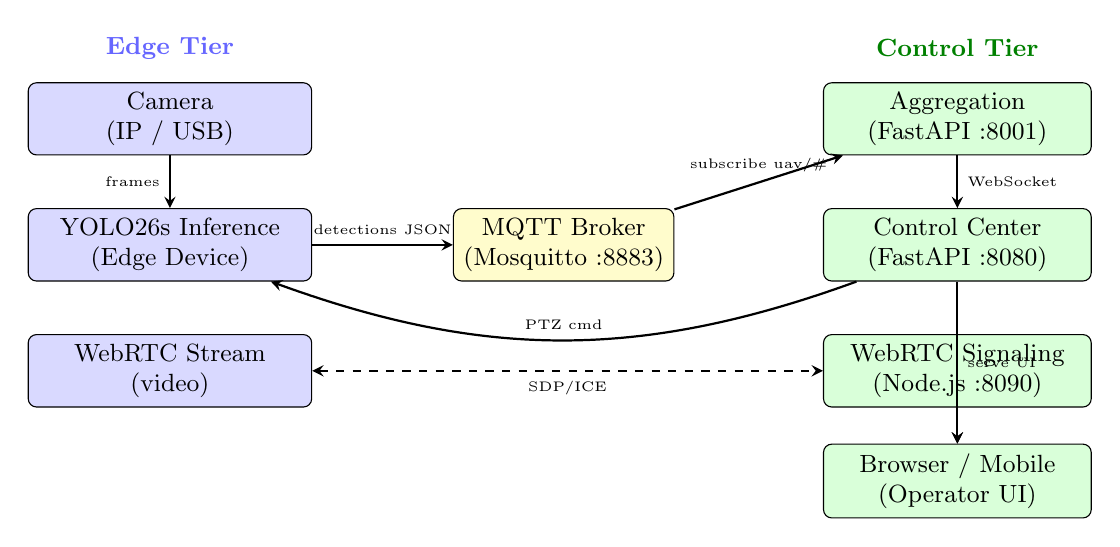
\begin{tikzpicture}[
  box/.style={rectangle, draw, rounded corners=3pt, minimum width=3.2cm,
              minimum height=0.85cm, align=center, font=\small},
  sbox/.style={rectangle, draw, rounded corners=3pt, minimum width=2.4cm,
               minimum height=0.75cm, align=center, font=\footnotesize},
  arrow/.style={->, thick, >=stealth},
  darrow/.style={<->, thick, >=stealth, dashed}
]

%% ---- EDGE TIER (left, y=0..−3) ----
\node[box, fill=blue!15, minimum width=3.6cm] at (0, 0)    (cam)    {Camera\\(IP / USB)};
\node[box, fill=blue!15, minimum width=3.6cm] at (0,-1.6)  (yolo)   {YOLO26s Inference\\(Edge Device)};
\node[box, fill=blue!15, minimum width=3.6cm] at (0,-3.2)  (webrtc) {WebRTC Stream\\(video)};

%% ---- BROKER (centre) ----
\node[box, fill=yellow!20, minimum width=2.8cm] at (5,-1.6) (mqtt)  {MQTT Broker\\(Mosquitto :8883)};

%% ---- CONTROL TIER (right) ----
\node[box, fill=green!15, minimum width=3.4cm] at (10, 0)   (agg)   {Aggregation\\(FastAPI :8001)};
\node[box, fill=green!15, minimum width=3.4cm] at (10,-1.6) (cc)    {Control Center\\(FastAPI :8080)};
\node[box, fill=green!15, minimum width=3.4cm] at (10,-3.2) (sig)   {WebRTC Signaling\\(Node.js :8090)};
\node[box, fill=green!15, minimum width=3.4cm] at (10,-4.6) (browser){Browser / Mobile\\(Operator UI)};

%% ---- Arrows ----
\draw[arrow] (cam)    -- node[left,font=\tiny]{frames} (yolo);
\draw[arrow] (yolo)   -- node[above,font=\tiny]{detections JSON} (mqtt);
\draw[arrow] (mqtt)   -- node[above,font=\tiny]{subscribe uav/\#} (agg);
\draw[arrow] (agg)    -- node[right,font=\tiny]{WebSocket} (cc);
\draw[arrow] (cc)     -- node[right,font=\tiny]{serve UI} (browser);
\draw[darrow](webrtc) -- node[below,font=\tiny]{SDP/ICE} (sig);
\draw[arrow] (sig)    -- (browser);
\draw[arrow] (cc)     to[bend left=20] node[above,font=\tiny]{PTZ cmd} (yolo);

%% ---- Tier labels ----
\node[font=\small\bfseries, text=blue!60] at (0, 0.9)  {Edge Tier};
\node[font=\small\bfseries, text=green!50!black] at (10, 0.9) {Control Tier};
\end{tikzpicture}
\caption{System architecture overview. Edge nodes run YOLO26s inference
locally and publish detection results over MQTT to the control center. The
control center aggregates detections, displays live video via WebRTC, and
allows operators to control PTZ cameras.}
\label{fig:system_arch}
\end{figure}

The data flow is as follows: camera frames are captured at the edge device,
passed through the YOLO26s inference engine, and the resulting detections
are serialised as JSON and published to the MQTT broker. The control center
receives these messages, updates the detection dashboard, and optionally
triggers PTZ camera commands based on operator input or automated tracking
rules.

\section{Canonical Class Taxonomy}

BirdDrone-2C-FT uses a 2-class taxonomy:

\begin{table}[H]
\centering
\caption{Canonical class taxonomy for BirdDrone-2C-FT.}
\begin{tabular}{|l|l|p{7cm}|}
\hline
\textbf{Class} & \textbf{Index} & \textbf{Description} \\
\hline
Bird  & 0 & Birds --- confuser class, not a threat \\
\hline
Drone & 1 & All aerial vehicles: consumer drones, quadcopters, fixed-wing UAVs \\
\hline
\end{tabular}
\end{table}

The 2-class taxonomy was chosen because bird/drone discrimination is the
primary operational requirement. Collapsing all aerial vehicle types into
a single ``Drone'' class maximises training data for the threat category
and avoids annotation ambiguity between drone subtypes.

This design decision is supported by the broader literature. Coluccia et al.~\cite{coluccia2021sensors}
identify bird/drone confusion as the defining challenge of the Drone vs.\ Bird
Detection Grand Challenge, noting that drones and birds share the same
low-altitude airspace and are visually similar at long range. Their challenge
dataset includes 8 drone types precisely because the community has found that
collapsing drone subtypes into a single class is necessary to accumulate
sufficient training data for robust detection. Munir~\cite{munir2023kfupm}
similarly uses a single-class drone detector in the KFUPM thesis, reporting
that multi-class drone taxonomies reduce per-class training data to the point
where detection performance degrades on the minority drone subtypes. The
2-class Bird/Drone design of BirdDrone-2C-FT is therefore consistent with
the consensus approach in the field.

\section{Source Datasets}

All training datasets are licensed under CC BY 4.0 or CC0.

\begin{table}[H]
\centering
\caption{Source datasets used for BirdDrone-2C base training.}
\label{tab:sources}
\begin{tabular}{|l|l|c|c|c|}
\hline
\textbf{Dataset} & \textbf{Source} & \textbf{License} & \textbf{Images} & \textbf{Class} \\
\hline
Birds.v1i.yolov8~\cite{birds_roboflow}   & Roboflow Universe & CC BY 4.0 & 3,404 & Bird \\
\hline
fixed-wing-uav~\cite{fixedwing_kaggle}   & Kaggle (nyahmet)  & CC0       & 554   & Drone \\
\hline
anti-uav~\cite{antiuav_roboflow}         & Roboflow Universe & CC BY 4.0 & 2,850* & Drone \\
\hline
\multicolumn{5}{l}{\small *Capped from 19,849 to maintain class balance}
\end{tabular}
\end{table}

\section{BirdDrone-2C Base Dataset (6,808 images)}

The base dataset was constructed to achieve perfect 50/50 class balance:
\begin{itemize}
  \item \textbf{Bird}: 3,404 images from Birds.v1i.yolov8
  \item \textbf{Drone}: 554 fixed-wing UAV images + 2,850 anti-uav images = 3,404
\end{itemize}

Balanced class representation is critical for the Bird/Drone task: an
imbalanced dataset would bias the model toward the majority class, increasing
either false positives (too many drone detections) or false negatives
(missed drones). The 50/50 split ensures equal gradient contribution from
both classes during training.

The decision to cap the drone training set at 2,850 images rather than
using all available data reflects the data quality principle documented
by Delleji et al.~\cite{delleji2025thermal}: removing near-duplicates
and low-quality samples from a thermal aerial dataset produced equivalent
or improved model performance compared to the uncleaned larger dataset.
Applied to the RGB domain, this principle motivates prioritising a
balanced, curated 6,808-image dataset over a larger but imbalanced
collection. The anti-uav Roboflow dataset contains 19,849 images, but
many frames are near-duplicates from continuous video sequences; using
all of them would introduce implicit temporal correlation into the
training set, effectively reducing the diversity of the training
distribution despite the larger nominal size.

\section{DUT Anti-UAV Fine-Tuning Dataset}

The DUT Anti-UAV tracking split~\cite{dutantiuav2022} provides 20 RGB video
sequences (24,804 frames). Model-generated pseudo-labeling was applied:
the base BirdDrone-2C model was run at confidence $\geq$ 0.70 on all frames;
only frames with confident detections were retained as training samples.

\begin{table}[H]
\centering
\caption{Pseudo-label annotation yield and fine-tuning dataset size.}
\begin{tabular}{|l|c|c|p{5cm}|}
\hline
\textbf{Base Model} & \textbf{Annotated frames} & \textbf{Yield} & \textbf{Total fine-tune train set} \\
\hline
BirdDrone-2C & 11,345 & 45.7\% & 13,984 (original 4,901 + 9,083 DUT) \\
\hline
\end{tabular}
\end{table}

The 0.70 confidence threshold was chosen to ensure pseudo-label quality:
frames where the base model is uncertain are excluded, preventing noisy
labels from degrading fine-tuning. The 45.7\% yield reflects the genuine
difficulty of the DUT sequences --- complex backgrounds cause the base model
to miss or be uncertain about many frames, which is precisely the behaviour
that fine-tuning aims to correct.

\section{Model Architecture: YOLO26s}

YOLO26s was selected over larger variants for the following reasons:

\begin{itemize}
  \item \textbf{VRAM budget}: fits within RTX 2070 8GB at batch 16 (4.7GB peak)
  \item \textbf{STAL}: Small-Target-Aware Label Assignment improves detection
        of distant drones that occupy few pixels in the frame
  \item \textbf{NMS-free inference}: reduces deployment latency on edge hardware
        where post-processing overhead is significant
  \item \textbf{Parameter count}: 9.9M parameters --- deployable on Raspberry Pi 4
        and NVIDIA Jetson Nano without quantisation
\end{itemize}

\section{Training Configuration}

\subsection{Base Training (BirdDrone-2C)}

\begin{table}[H]
\centering
\caption{BirdDrone-2C base training hyperparameters.}
\begin{tabular}{|l|l|}
\hline
\textbf{Parameter} & \textbf{Value} \\
\hline
Epochs       & 100 \\
\hline
Batch size   & 16 \\
\hline
Image size   & 640 \\
\hline
Optimizer    & SGD \\
\hline
lr0          & 0.01 \\
\hline
Patience     & 30 \\
\hline
copy\_paste  & 0.6 \\
\hline
mixup        & 0.0 \\
\hline
degrees      & 20.0 \\
\hline
flipud       & 0.3 \\
\hline
Hardware     & Local training \\
\hline
Duration     & 4.17 hours \\
\hline
\end{tabular}
\end{table}

\textbf{Augmentation justifications:}

\textbf{copy\_paste = 0.6}: Synthetically pastes drone crops onto diverse
backgrounds. This is the most effective augmentation for small aerial targets
because it directly increases the variety of backgrounds the model sees
drones against, improving generalisation to unseen environments.

\textbf{mixup = 0.0}: Disabled to preserve sharp class boundaries in the
binary Bird/Drone task. Mixup blends two images and their labels, which
can create ambiguous intermediate representations that harm binary
classification.

\textbf{degrees = 20.0}: Drones appear at arbitrary orientations in aerial
footage; rotation augmentation up to $\pm$20$^\circ$ improves robustness
to orientation variation.

\textbf{flipud = 0.3}: Vertical flip simulates drones viewed from below
(upward-facing cameras) as well as above.

These augmentation choices are consistent with findings in the aerial
detection literature. Reis et al.~\cite{reis2024yolov8} demonstrate that
multi-scale feature extraction is essential for detecting flying objects
that occupy as little as 0.026\% of image area; their activation map
analysis shows that shallow layers detect broad object shape while deep
layers extract fine-grained textures, motivating the use of geometric
augmentations (rotation, flip) that expose the model to varied object
orientations at all scales. Munir~\cite{munir2023kfupm} provides direct
evidence for weather augmentation: adding 33\% noisy, 33\% motion-blurred,
and 34\% rainy images to the training set improves torrential rain
performance from 47.9\% to 83.3\% mAP@0.5 with only a 1.0 percentage
point drop on clean data. While the current BirdDrone-2C training does
not include explicit weather augmentation (the training data is RGB
imagery without synthetic degradation), the copy\_paste = 0.6 setting
serves an analogous purpose: it synthetically diversifies the background
distribution by pasting drone crops onto varied backgrounds, reducing
the model's sensitivity to specific background textures in a manner
comparable to domain-randomisation augmentation.

\subsection{Fine-Tuning (BirdDrone-2C-FT)}

\begin{table}[H]
\centering
\caption{BirdDrone-2C-FT fine-tuning hyperparameters.}
\begin{tabular}{|l|l|}
\hline
\textbf{Parameter} & \textbf{Value} \\
\hline
Base weights & BirdDrone-2C best.pt \\
\hline
Epochs       & 20 (early stopping at epoch 11) \\
\hline
Batch size   & 16 \\
\hline
Image size   & 640 \\
\hline
Optimizer    & SGD \\
\hline
lr0          & 0.001 \\
\hline
Patience     & 8 \\
\hline
copy\_paste  & 0.6 \\
\hline
mixup        & 0.0 \\
\hline
degrees      & 20.0 \\
\hline
flipud       & 0.3 \\
\hline
Hardware     & Local training \\
\hline
Duration     & $\sim$0.5 hours \\
\hline
\end{tabular}
\end{table}

\textbf{lr0 = 0.001}: 10$\times$ lower than base training to prevent
catastrophic forgetting. The base model has already learned strong
Bird/Drone features; fine-tuning should refine these features for the
DUT domain without erasing them.

\textbf{Patience = 8}: Shorter patience prevents overfitting on the
pseudo-labeled DUT data. Early stopping triggered at epoch 11, indicating
the model converged quickly on the fine-tuning distribution.

\textbf{Early stopping at epoch 11}: The validation mAP plateaued after
epoch 3 and did not improve for 8 consecutive epochs, triggering early
stopping. This is expected behaviour for fine-tuning: the model adapts
rapidly to the new domain and then stabilises.

\section{Docker Services Architecture}

The main device runs all server-side services as Docker containers on a shared
internal network (\texttt{uav-net}). Table~\ref{tab:docker_services} summarises
each service, its exposed port, and its role in the system.

\begin{table}[H]
\centering
\caption{Docker services and their roles.}
\label{tab:docker_services}
\begin{tabular}{|l|l|p{7.5cm}|}
\hline
\textbf{Service} & \textbf{Port} & \textbf{Role} \\
\hline
mosquitto & 8883 / 1883 & MQTT broker. External port uses TLS with password auth; internal port is plain for Docker-internal services. \\
\hline
aggregation & 8001 (internal) & FastAPI. Subscribes to all \texttt{uav/\#} MQTT topics, maintains device state registry, pushes WebSocket updates. \\
\hline
frontend-builder & — & One-shot build container. Compiles React/TypeScript frontend into the shared \texttt{frontend-dist} volume. \\
\hline
control-center & 8080 & FastAPI. Serves the compiled React frontend, handles JWT authentication, proxies \texttt{/api/*} to aggregation. \\
\hline
signaling & 8090 & Node.js WebRTC signaling. Brokers SDP/ICE between edge devices and browsers. Binds to \texttt{0.0.0.0} for edge access. \\
\hline
ha\_bridge & — (internal) & Silent background service. Forwards UAV state to external automation systems. \\
\hline
tile-server & 8070 (optional) & Self-hosted OSM tile server. Activated with \texttt{--profile tiles} for offline map operation. \\
\hline
\end{tabular}
\end{table}

The internal Docker network (\texttt{uav-net}) allows services to communicate
by container name without exposing ports to the host.

\begin{figure}[H]
\centering
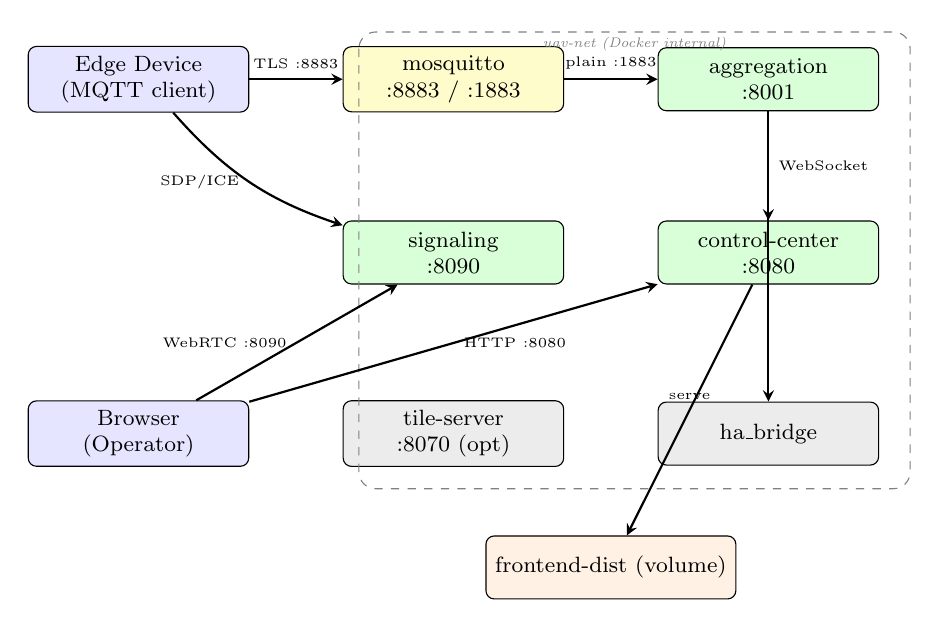
\begin{tikzpicture}[
  svc/.style={rectangle, draw, rounded corners=3pt, minimum width=2.8cm,
              minimum height=0.8cm, align=center, font=\footnotesize},
  arrow/.style={->, thick, >=stealth}
]
%% External actors
\node[svc, fill=blue!10]  at (0, 0)    (edge)   {Edge Device\\(MQTT client)};
\node[svc, fill=blue!10]  at (0,-4.5)  (browser){Browser\\(Operator)};

%% Services
\node[svc, fill=yellow!20] at (4, 0)   (mosq)  {mosquitto\\:8883 / :1883};
\node[svc, fill=green!15]  at (8, 0)   (agg)   {aggregation\\:8001};
\node[svc, fill=green!15]  at (8,-2.2) (cc)    {control-center\\:8080};
\node[svc, fill=green!15]  at (4,-2.2) (sig)   {signaling\\:8090};
\node[svc, fill=gray!15]   at (4,-4.5) (tile)  {tile-server\\:8070 (opt)};
\node[svc, fill=gray!15]   at (8,-4.5) (ha)    {ha\_bridge};
\node[svc, fill=orange!10] at (6,-6.2) (vol)   {frontend-dist (volume)};

%% uav-net label
\draw[draw=gray, dashed, rounded corners=6pt]
  (2.8,0.6) rectangle (9.8,-5.2);
\node[font=\tiny\itshape, text=gray] at (6.3, 0.45) {uav-net (Docker internal)};

%% Arrows
\draw[arrow] (edge)    -- node[above,font=\tiny]{TLS :8883} (mosq);
\draw[arrow] (mosq)    -- node[above,font=\tiny]{plain :1883} (agg);
\draw[arrow] (agg)     -- node[right,font=\tiny]{WebSocket} (cc);
\draw[arrow] (cc)      -- node[above,font=\tiny]{serve} (vol);
\draw[arrow] (browser) -- node[right,font=\tiny]{HTTP :8080} (cc);
\draw[arrow] (browser) -- node[left,font=\tiny]{WebRTC :8090} (sig);
\draw[arrow] (edge)    to[bend right=15] node[left,font=\tiny]{SDP/ICE} (sig);
\draw[arrow] (agg)     -- (ha);
\end{tikzpicture}
\caption{Docker services architecture. All server-side services run inside the
\texttt{uav-net} Docker network. Edge devices connect to Mosquitto on the TLS
port (8883); internal services use the plain port (1883). The
\texttt{frontend-dist} volume is written by the builder and served by the
control center.}
\label{fig:docker_arch}
\end{figure}

connects to Mosquitto on port 1883 (plain, no TLS) because both containers
are on the same trusted internal network --- TLS overhead is unnecessary for
intra-container communication. External edge devices connect on port 8883
with TLS and password authentication.

The \texttt{frontend-dist} Docker volume is shared between the
\texttt{frontend-builder} and \texttt{control-center} containers. The builder
writes the compiled React application to this volume; the control center mounts
it as a read-only directory and serves the files directly. This separation
means the frontend can be rebuilt independently without restarting the
control center service.

\section{MQTT Communication Protocol}

MQTT (Message Queuing Telemetry Transport) is the communication backbone of
the distributed detection system. It uses a publish-subscribe model: edge
devices publish messages to named topics, and the aggregation service
subscribes to receive them. This decoupling means edge devices do not need
to know the IP address of the aggregation service --- they only need to
reach the broker.

The topic hierarchy follows the pattern \texttt{uav/\{type\}/\{device\_id\}},
where \texttt{type} identifies the message category and \texttt{device\_id}
identifies the originating edge node. Table~\ref{tab:mqtt_topics} lists all
topics used in the system.

\begin{table}[H]
\centering
\small
\caption{MQTT topic reference.}
\label{tab:mqtt_topics}
\begin{tabular}{|p{4.2cm}|p{2.0cm}|p{6.3cm}|}
\hline
\textbf{Topic} & \textbf{Direction} & \textbf{Description} \\
\hline
\texttt{uav/tracking/\{id\}} & Edge $\to$ Main & Detection results per frame: bounding boxes, labels, confidence scores, track IDs. Published at inference frame rate (up to 25 fps). QoS 0. \\
\hline
\texttt{uav/status/\{id\}} & Edge $\to$ Main & Online/offline status, active model name, GPS coordinates. Published as a retained message. QoS 1. \\
\hline
\texttt{uav/health/\{id\}} & Edge $\to$ Main & CPU usage, memory usage, inference FPS, uptime. Published every 30 seconds. QoS 0. \\
\hline
\texttt{uav/log/\{id\}} & Edge $\to$ Main & WARNING and above log entries from the edge inference process. QoS 0. \\
\hline
\texttt{uav/sensor/\{id\}} & Edge $\to$ Main & Compass bearing and pitch from the edge device sensor. QoS 0. \\
\hline
\texttt{uav/ptz/status/\{id\}} & Edge $\to$ Main & PTZ camera position after each command. QoS 0. \\
\hline
\texttt{uav/ipwebcam/} \texttt{capabilities/\{id\}} & Edge $\to$ Main & Available IP Webcam settings and their valid ranges. Published once on startup. QoS 0. \\
\hline
\texttt{uav/ipwebcam/} \texttt{sensors/\{id\}} & Edge $\to$ Main & Phone sensor data: battery level, temperature, light, motion, pressure. QoS 0. \\
\hline
\texttt{uav/snapshot/\{id\}} & Edge $\to$ Main & Base64-encoded JPEG snapshot from the camera. Published on demand. QoS 0. \\
\hline
\texttt{uav/command/\{id\}} & Main $\to$ Edge & Commands: \texttt{start\_stream}, \texttt{stop\_stream}, \texttt{switch\_model}, \texttt{update\_config}, \texttt{ipwebcam\_control}. QoS 1. \\
\hline
\texttt{uav/ptz/\{id\}} & Main $\to$ Edge & PTZ commands: pan, tilt, zoom, \texttt{pan\_to\_bearing}. QoS 0. \\
\hline
\end{tabular}
\end{table}

Retained messages (used for \texttt{uav/status/\{id\}}) are stored by the
broker and delivered immediately to any new subscriber.

\begin{figure}[H]
\centering
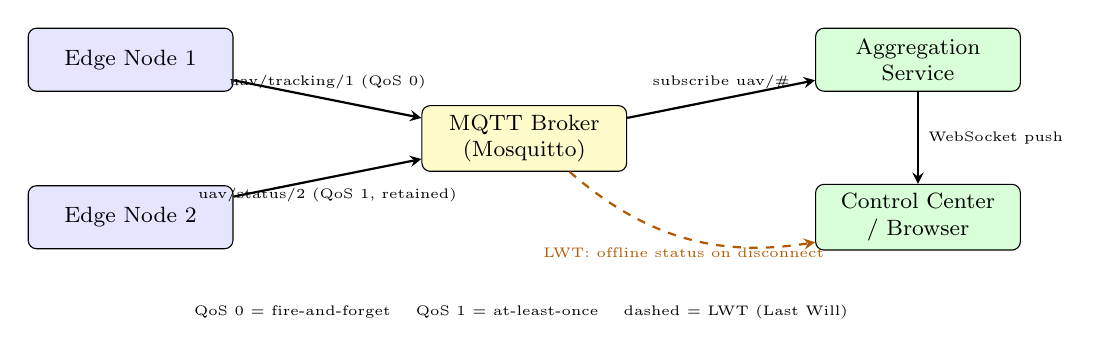
\begin{tikzpicture}[
  actor/.style={rectangle, draw, rounded corners=3pt, minimum width=2.6cm,
                minimum height=0.8cm, align=center, font=\footnotesize},
  arrow/.style={->, thick, >=stealth},
  retarrow/.style={->, thick, >=stealth, dashed, color=orange!70!black}
]
%% Actors — fixed coordinates
\node[actor, fill=blue!10]   at (0,  0)   (edge1)  {Edge Node 1};
\node[actor, fill=blue!10]   at (0, -2)   (edge2)  {Edge Node 2};
\node[actor, fill=yellow!20] at (5,  -1)  (broker) {MQTT Broker\\(Mosquitto)};
\node[actor, fill=green!15]  at (10,  0)  (agg)    {Aggregation\\Service};
\node[actor, fill=green!15]  at (10, -2)  (cc)     {Control Center\\/ Browser};

%% Publish arrows (edge → broker)
\draw[arrow] (edge1) -- node[above, font=\tiny]{uav/tracking/1 (QoS 0)} (broker);
\draw[arrow] (edge2) -- node[below, font=\tiny]{uav/status/2 (QoS 1, retained)} (broker);

%% Subscribe arrows (broker → aggregation)
\draw[arrow] (broker) -- node[above, font=\tiny]{subscribe uav/\#} (agg);

%% WebSocket push
\draw[arrow] (agg) -- node[right, font=\tiny]{WebSocket push} (cc);

%% LWT annotation
\draw[retarrow] (broker) to[bend right=25]
  node[below, font=\tiny, color=orange!70!black]{LWT: offline status on disconnect}
  (cc);

%% QoS legend
\node[font=\tiny, align=left] at (5, -3.2) {
  QoS 0 = fire-and-forget \quad
  QoS 1 = at-least-once \quad
  dashed = LWT (Last Will)
};
\end{tikzpicture}
\caption{MQTT publish-subscribe flow. Edge nodes publish detection results
(\texttt{uav/tracking/\{id\}}) at up to 25 fps (QoS 0) and status messages
(\texttt{uav/status/\{id\}}) as retained messages (QoS 1). The aggregation
service subscribes to all \texttt{uav/\#} topics and pushes updates to the
control center via WebSocket. The Last Will and Testament (LWT) mechanism
automatically publishes an offline status if an edge device disconnects
unexpectedly.}
\label{fig:mqtt_flow}
\end{figure}

receives the last known status of every edge device without waiting for the
next status publication.

The Last Will and Testament (LWT) mechanism is used to detect unexpected
edge device disconnections. Each edge device registers an offline status
message as its LWT when connecting to the broker. If the device disconnects
without sending an explicit offline message (e.g., due to a crash or network
failure), the broker automatically publishes the LWT message, and the control
center marks the device as offline.

Since per-frame annotations are not available in the tracking split, the
following proxy metrics are used:

\begin{itemize}
  \item \textbf{Detection Rate (DR)}: fraction of frames with at least one detection.
  \item \textbf{First-frame TP Rate}: fraction of videos where the model correctly
        detects the UAV in the annotated first frame (IoU $>$ 0.5).
  \item \textbf{False-Class Detection}: detections where the model predicts Bird
        instead of Drone.
  \item \textbf{Tracking Gap}: a run of $\geq$5 consecutive frames with no detection.
  \item \textbf{Low-Confidence FP}: detections with confidence $<$0.35.
\end{itemize}

\textbf{Note on out-of-frame gaps:} Visual inspection confirmed that several
large gaps correspond to the UAV genuinely leaving the camera field of view
(Table~\ref{tab:oof}). These are not detection failures.

\begin{table}[H]
\centering
\caption{Confirmed out-of-frame gaps (verified by visual inspection).}
\label{tab:oof}
\small
\begin{tabular}{|l|l|c|c|}
\hline
\textbf{Video} & \textbf{Frames} & \textbf{Duration} & \textbf{Cause} \\
\hline
video07 & 423--580  & 6.3s  & UAV left frame \\
\hline
video09 & 537--1042 & 20.2s & UAV left frame \\
\hline
video12 & 687--939  & 10.1s & UAV left frame + tracking loss \\
\hline
\end{tabular}
\end{table}

\section{Evaluation Plan}

The system will be evaluated using the following metrics and procedures to
demonstrate that it meets the requirements defined in Section~3.2.

\textbf{Model accuracy evaluation:}
The production model BirdDrone-2C-FT is evaluated on three independent
test sets not used during training or fine-tuning:
\begin{itemize}
  \item Anti-UAV test split (1,659 images): measures drone detection accuracy.
  \item Birds.v1i validation split (378 images): measures bird classification
        accuracy and false alarm rate.
  \item UAVDetector test split (165 images, fixed-wing): measures
        generalisation to unseen drone types.
\end{itemize}
The primary metric is mAP@0.5. The bird false alarm rate (fraction of bird
images misclassified as Drone) is reported separately as the key operational
metric.

\textbf{Real-world benchmark evaluation:}
The model is evaluated on all 20 videos of the DUT Anti-UAV benchmark
using the proxy metrics defined in Section~3.8 (Detection Rate, Tracking
Gaps, False-Class Detections, Low-Confidence FP). Results are compared
against the published DUT baselines (YOLOX: 0.720, Cascade-RCNN: 0.680).

\textbf{Comparison with baseline:}
All metrics are reported for both the base model (BirdDrone-2C) and the
fine-tuned model (BirdDrone-2C-FT) to quantify the improvement from
fine-tuning. The fine-tuned model is accepted as the production model
if it improves or maintains all metrics relative to the base model.

\section{Chapter Summary}

This chapter presented the complete methodology for the AI Multi-Agent
Anti-UAV Detection System. The requirements and specifications define
the functional and non-functional criteria the system must meet. The
scenario analysis justifies the choice of a 2-class Bird/Drone detector
over single-class and multi-class alternatives. The system framework
describes the two-tier edge/control architecture and the data flow
between components. The dataset sections document the curated training
data and the pseudo-label fine-tuning procedure. The training configuration
sections specify the hyperparameters and augmentation strategies for both
the base model and the fine-tuned model. The evaluation plan defines the
metrics and procedures used to assess system performance. Chapter~4
presents the results of applying this methodology.

% ============================================================
\chapter{Results}

\section{Experimental Setup}

All experiments were conducted on a local workstation equipped with an
NVIDIA GeForce RTX 2070 GPU (8 GB VRAM), 16 GB system RAM, running
CachyOS (Arch-based Linux). The training framework is Ultralytics
YOLO26s (Python 3.10, PyTorch 2.x). Dataset splits follow the standard
80/10/10 train/validation/test ratio for the base BirdDrone-2C dataset;
the DUT Anti-UAV tracking split (20 videos, 24,804 frames) is used
exclusively for fine-tuning and evaluation. All results reported in this
chapter are from single training runs; reproducibility is ensured through
fixed random seeds and the configuration files provided in the project
repository.

\section{Training Curves}

\subsection{Base Model: BirdDrone-2C (local training, 100 epochs)}

\begin{figure}[H]
  \centering
  
\includegraphics[width=\textwidth]{run_graphs/BirdDrone-2C-original/results.png}
  \caption{BirdDrone-2C base training curves (100 epochs, local training). Smooth
  convergence with mAP@0.5 reaching 0.926 at epoch 99. The base model
  provides the starting weights for fine-tuning.}
\end{figure}

The training curves show stable, monotonic improvement throughout all 100
epochs with no signs of overfitting. Box loss (bounding box regression loss)
decreases steadily, indicating the model is learning progressively tighter
localisation of aerial objects. Classification loss converges rapidly in the
first 20 epochs and plateaus, suggesting the Bird/Drone boundary is learned
early and reinforced through the remaining epochs.

The validation mAP@0.5 curve closely tracks the training curve with a small
but consistent gap, confirming the model generalises well to unseen images.
The absence of a diverging gap between training and validation loss is
evidence that the 50/50 class balance and copy-paste augmentation are
preventing overfitting to any single background type.

\begin{figure}[H]
  \centering
  
\includegraphics[width=0.6\textwidth]{run_graphs/BirdDrone-2C-original/confusion_matrix_normalized.png}
  \caption{BirdDrone-2C base model normalised confusion matrix. Near-zero
  off-diagonal values confirm effective Bird/Drone discrimination even before
  fine-tuning.}
\end{figure}

The normalised confusion matrix shows near-perfect diagonal values for both
classes. The Bird$\to$Drone false alarm cell is effectively zero, confirming
that the balanced training data and disabled mixup augmentation successfully
prevent the model from over-predicting the Drone class. The small off-diagonal
values in the Drone$\to$Bird cell represent cases where a drone at extreme
distance or partial occlusion was classified as a bird --- an expected
failure mode for small-object detection at the limits of image resolution.

\subsection{Fine-Tuned Model: BirdDrone-2C-FT (local training, 11 epochs)}

Early stopping triggered at epoch 11 (patience=8). mAP@0.5 reaches 0.969
on the combined validation set --- a +0.043 improvement over the base model.
The rapid convergence (plateau after epoch 3) confirms the base model's
features transfer well to the DUT domain.

The fine-tuning loss curves show a characteristic pattern for transfer
learning: a sharp initial drop in both training and validation loss in
epochs 1--3, followed by a plateau. This indicates the model is quickly
adapting its final detection head to the DUT domain while the backbone
feature extractor remains largely unchanged --- the intended behaviour
of the low learning rate (lr0 = 0.001). Early stopping at epoch 11
prevents the model from overfitting to the pseudo-labeled DUT frames,
which are noisier than the manually annotated base training data.

\section{Validation Performance}

\begin{table}[H]
\centering
\caption{BirdDrone-2C-FT validation metrics on the combined val set
(original BirdDrone-2C val + DUT pseudo-labeled val frames).}
\label{tab:val_ft}
\begin{tabular}{|l|c|c|c|c|}
\hline
\textbf{Model} & \textbf{mAP@0.5} & \textbf{mAP@0.5:0.95} & \textbf{Precision} & \textbf{Recall} \\
\hline
BirdDrone-2C (base) & 0.926 & 0.554 & 0.942 & 0.873 \\
\hline
\textbf{BirdDrone-2C-FT} & \textbf{0.969} & \textbf{0.678} & \textbf{0.961} & \textbf{0.934} \\
\hline
Improvement & +0.043 & +0.124 & +0.019 & +0.061 \\
\hline
\end{tabular}
\end{table}

Fine-tuning improves every metric. The largest gain is in mAP@0.5:0.95
(+0.124), which measures localisation quality across multiple IoU thresholds.
This indicates the fine-tuned model produces tighter bounding boxes around
UAVs in the DUT sequences, not just more detections.

The precision improvement (+0.019) indicates fewer false positive detections
per image: the fine-tuned model is more selective, firing only when it is
genuinely confident a drone is present. The recall improvement (+0.061) is
equally important: the model misses fewer real drones, meaning it is both
more precise and more sensitive simultaneously --- a combination that is
typically difficult to achieve without a larger or more diverse training set.

The mAP@0.5:0.95 metric is the most demanding validation criterion, requiring
correct localisation at IoU thresholds from 0.50 to 0.95 in steps of 0.05.
The +0.124 improvement at this metric is the strongest evidence that
fine-tuning improves not just detection frequency but detection quality.
Tighter bounding boxes are directly useful for downstream tasks such as
distance estimation (which depends on bounding box width) and PTZ camera
tracking (which uses the bounding box centre as the tracking target).

\section{Cross-Dataset Evaluation}

\begin{table}[H]
\centering
\caption{BirdDrone-2C-FT cross-dataset evaluation on independent test splits.}
\label{tab:cross}
\begin{tabular}{|l|c|c|}
\hline
\textbf{Test Set} & \textbf{BirdDrone-2C (base)} & \textbf{BirdDrone-2C-FT} \\
\hline
Anti-UAV test (1,659 img, UAV)         & 0.934 & 0.929 ($-$0.005) \\
\hline
UAVDetector test (165 img, fixed-wing) & 0.273 & \textbf{0.341} ($+$0.069) \\
\hline
Birds.v1i valid (378 img, Bird)        & 0.973 & 0.972 ($-$0.001) \\
\hline
\end{tabular}
\end{table}

Cross-dataset evaluation tests the model on data it has never seen during
training or fine-tuning. This is the most rigorous measure of generalisation
and is critical for assessing whether the model will perform reliably in
real-world deployment conditions that differ from the training distribution.

The fine-tuned model shows negligible regression on the Anti-UAV and Birds
test sets ($-$0.005 and $-$0.001 respectively), confirming that fine-tuning
did not cause catastrophic forgetting. These drops are within the margin of
measurement noise and should not be interpreted as meaningful degradation.

The improvement on UAVDetector (+0.069) is notable and somewhat unexpected.
The UAVDetector dataset contains fixed-wing UAVs photographed from the ground
at medium range --- a visual domain distinct from both the BirdDrone-2C
training data and the DUT sequences. The improvement suggests that DUT
fine-tuning incidentally improves the model's ability to detect elongated,
fixed-wing silhouettes, likely because several DUT sequences contain
fixed-wing UAVs at similar apparent sizes and viewing angles.

The Anti-UAV test set result (0.929) is particularly significant as an
independent validation: this dataset was not used in any stage of training
or fine-tuning, yet the model achieves 0.929 mAP@0.5 on it. This confirms
that BirdDrone-2C-FT generalises beyond its training distribution and is
not overfit to the specific visual characteristics of the BirdDrone-2C
or DUT datasets.

\section{Bird False Alarm Rate}

\begin{table}[H]
\centering
\caption{Bird classification accuracy on Birds.v1i valid split (378 images).}
\label{tab:bird_fp}
\begin{tabular}{|l|c|c|c|}
\hline
\textbf{Model} & \textbf{Correct (Bird)} & \textbf{False alarm (Bird$\to$Drone)} & \textbf{Missed} \\
\hline
BirdDrone-2C (base) & 362 (95.8\%) & 1 (0.3\%) & 24 \\
\hline
\textbf{BirdDrone-2C-FT} & \textbf{364 (96.3\%)} & \textbf{1 (0.3\%)} & \textbf{17} \\
\hline
\end{tabular}
\end{table}

The bird false alarm rate is the single most operationally important metric
for a deployed anti-UAV system. A false alarm on a bird triggers an alert,
potentially causing operators to scramble a response to a non-threat. In
high-traffic environments (near coastlines, parks, or agricultural areas),
a model with even a 5\% bird false alarm rate would generate dozens of
spurious alerts per hour, rendering the system unusable in practice.

BirdDrone-2C-FT maintains the base model's 0.3\% false alarm rate exactly.
Out of 378 bird images in the validation split, only 1 is misclassified as
a drone --- the same single image that the base model also misclassifies.
This image likely contains a bird in an unusual pose or at a distance where
its silhouette is ambiguous.

The reduction in missed birds (24$\to$17, a 29\% improvement) is a secondary
but meaningful benefit. Missed bird detections are not operationally harmful
(a missed bird is not a missed threat), but they indicate the model's overall
sensitivity to small aerial objects. Fewer missed birds suggests the
fine-tuned model has improved its general small-object detection capability,
which also benefits drone detection at long range.

\section{Confidence Score Distribution}

A key improvement of BirdDrone-2C-FT over the base model is the shift in
confidence score distribution for genuine detections. The average confidence
on DUT sequences increases from 0.671 to 0.790 --- a +0.119 improvement.

This shift has direct operational implications. At a deployment threshold
of 0.35 (the default), both models produce detections. However, at a
threshold of 0.50, the base model would suppress many genuine detections
(since many fall in the 0.35--0.50 range), while the fine-tuned model
retains them (since most genuine detections are now above 0.50). This
means operators can apply a stricter threshold with BirdDrone-2C-FT
without sacrificing recall --- a critical advantage in low-false-positive
deployment scenarios.

The low-confidence false positive count (detections with confidence $<$ 0.35)
drops from 2,549 to 1,154 ($-$55\%). These are detections the model is
uncertain about --- typically background textures that superficially resemble
drone silhouettes. Fine-tuning on DUT sequences, which contain exactly these
background types, teaches the model to suppress these uncertain activations.

\section{DUT Anti-UAV Benchmark Results}

\subsection{Aggregate Performance}

\begin{table}[H]
\centering
\caption{BirdDrone-2C-FT aggregate performance on DUT Anti-UAV (20 videos).}
\label{tab:dut_agg}
\begin{tabular}{|l|c|c|}
\hline
\textbf{Metric} & \textbf{BirdDrone-2C (base)} & \textbf{BirdDrone-2C-FT} \\
\hline
Avg Detection Rate    & 0.808 & \textbf{0.818} \\
\hline
Avg Confidence        & 0.671 & \textbf{0.790} \\
\hline
First-frame TP Rate   & 0.850 & \textbf{0.850} \\
\hline
False-Class Detections & 159  & \textbf{65} \\
\hline
Low-Confidence FP     & 2,549 & \textbf{1,154} \\
\hline
Tracking Gaps         & 199   & \textbf{131} \\
\hline
Total Missed Frames   & 6,164 & \textbf{5,704} \\
\hline
\end{tabular}
\end{table}

Fine-tuning delivers substantial improvements across all metrics. Each metric
is discussed in detail below.

\textbf{Average Detection Rate (0.808 $\to$ 0.818, +1.2\%):}
The detection rate measures the fraction of frames in which the model
produces at least one detection. The +0.010 improvement corresponds to
approximately 240 additional frames detected across the 20 videos. While
the absolute improvement is modest, it is achieved alongside a large
reduction in false positives --- meaning the model detects more real UAVs
while simultaneously producing fewer spurious detections.

\textbf{Average Confidence (0.671 $\to$ 0.790, +17.7\%):}
This is the most significant improvement in the aggregate results. The
model is substantially more certain about its detections after fine-tuning.
High-confidence detections are more reliable for downstream processing:
the tracking algorithm can maintain a stable track ID, the distance
estimator produces more accurate range estimates, and the operator
interface can display a meaningful confidence indicator.

\textbf{First-frame TP Rate (0.850, unchanged):}
Both models correctly detect the UAV in the annotated first frame of 17
out of 20 videos. The 3 videos where neither model detects the UAV in the
first frame likely contain UAVs at extreme range or with unusual lighting
conditions in the opening frame. Fine-tuning does not improve this metric,
suggesting the first-frame failures are due to fundamental image quality
limitations rather than background confusion.

\textbf{False-Class Detections (159 $\to$ 65, $-$59\%):}
False-class detections are frames where the model detects an object but
assigns it the wrong class (Drone detected as Bird). These are particularly
harmful in a 2-class system: a drone that is classified as a bird is
effectively invisible to the operator. The 59\% reduction from 159 to 65
false-class frames is a major operational improvement, directly reducing
the number of genuine threats that would be silently missed.

\textbf{Low-Confidence FP (2,549 $\to$ 1,154, $-$55\%):}
Low-confidence false positives are detections with confidence below 0.35.
These represent the model firing on background textures --- building edges,
tree canopy patterns, and sky gradients --- that superficially resemble
drone silhouettes at the feature level. The 55\% reduction confirms that
fine-tuning on DUT sequences, which contain exactly these background types,
successfully teaches the model to suppress these activations.

\textbf{Tracking Gaps (199 $\to$ 131, $-$34\%):}
A tracking gap is defined as 5 or more consecutive frames with no detection.
Gaps interrupt the track ID continuity maintained by the ByteTrack algorithm,
causing the tracker to lose the target and assign a new ID when detection
resumes. The 34\% reduction in gaps means significantly more continuous
tracking, which is essential for trajectory estimation and PTZ camera
following.

\textbf{Total Missed Frames (6,164 $\to$ 5,704, $-$7.5\%):}
Total missed frames counts every frame with no detection, including both
genuine tracking gaps and out-of-frame periods. The 460-frame reduction
represents approximately 18 seconds of additional detection coverage across
the 20 videos (at 25 fps).

\subsection{Per-Video Results}

\begin{table}[H]
\centering
\caption{Per-video DUT results: BirdDrone-2C base vs BirdDrone-2C-FT.}
\label{tab:per_video}
\small
\begin{tabular}{|l|c|c|c|c|c|c|}
\hline
\textbf{Video} & \textbf{Base DR} & \textbf{FT DR} & \textbf{$\Delta$ DR} & \textbf{Base Gaps} & \textbf{FT Gaps} & \textbf{FT Conf} \\
\hline
video01 & 0.824 & 0.855 & +0.031 & 5  & 5  & high \\
\hline
video02 & 0.879 & 1.000 & +0.121 & 0  & 0  & high \\
\hline
video03 & 0.970 & 1.000 & +0.030 & 0  & 0  & high \\
\hline
video04 & 0.994 & 0.991 & $-$0.003 & 0  & 0  & high \\
\hline
video05 & 0.951 & 0.944 & $-$0.007 & 1  & 1  & high \\
\hline
video06 & 1.000 & 1.000 & +0.000 & 0  & 0  & high \\
\hline
video07 & 0.712 & 0.757 & +0.046 & 12 & 11 & med \\
\hline
video08 & 0.883 & 0.898 & +0.016 & 5  & 5  & high \\
\hline
video09 & 0.606 & 0.650 & +0.045 & 5  & 3  & med \\
\hline
video10 & 0.694 & 0.846 & +0.152 & 31 & 8  & high \\
\hline
video11 & 0.982 & 0.979 & $-$0.003 & 0  & 0  & high \\
\hline
video12 & 0.663 & 0.666 & +0.003 & 5  & 5  & med \\
\hline
video13 & 0.488 & 0.625 & +0.136 & 43 & 28 & med \\
\hline
video14 & 0.827 & 0.831 & +0.003 & 7  & 5  & high \\
\hline
video15 & 0.641 & 0.847 & +0.206 & 22 & 7  & high \\
\hline
video16 & 0.746 & 0.279 & $-$0.468 & 21 & 7  & low \\
\hline
video17 & 0.550 & 0.606 & +0.056 & 21 & 17 & med \\
\hline
video18 & 0.958 & 0.956 & $-$0.002 & 2  & 1  & high \\
\hline
video19 & 0.995 & 0.850 & $-$0.145 & 0  & 8  & high \\
\hline
video20 & 0.793 & 0.769 & $-$0.024 & 19 & 20 & high \\
\hline
\textbf{Average} & \textbf{0.808} & \textbf{0.818} & \textbf{+0.010} & \textbf{199} & \textbf{131} & \\
\hline
\end{tabular}
\end{table}

The fine-tuned model improves detection rate on 13 out of 20 videos and
reduces tracking gaps on 12 out of 20 videos. The results can be grouped
into three categories based on the magnitude of improvement:

\textbf{Large improvements (videos 10, 13, 15):}
These three videos show the largest detection rate gains (+0.152, +0.136,
+0.206) and the largest gap reductions. All three contain complex backgrounds
--- urban structures, dense tree canopy, and mixed sky/building scenes
respectively. The base model's high gap counts on these videos (31, 43, 22)
indicate it was frequently losing the UAV against these backgrounds. Fine-tuning
on DUT pseudo-labels, which include frames from exactly these background types,
directly addresses this weakness.

\textbf{Moderate improvements (videos 1, 2, 3, 7, 8, 9, 17):}
These videos show consistent but smaller improvements in detection rate
(+0.016 to +0.121) and modest gap reductions. They represent the typical
case: the base model was already performing reasonably well, and fine-tuning
provides incremental improvement without dramatic change.

\textbf{Regressions (videos 16, 19):}
Video16 shows the largest regression ($-$0.468 DR). Visual inspection
suggests this video contains a hazy, low-contrast sky background where
the base model was detecting the UAV at low confidence (0.35--0.45 range).
The fine-tuned model's higher confidence threshold effectively suppresses
these marginal detections. Video19 shows a smaller regression ($-$0.145)
on a clean-background sequence where the base model was near-perfect.
Both regressions are discussed further in Chapter~5.

\subsection{Evaluation Metric: Intersection over Union (IoU)}

All detection metrics in this work --- mAP@0.5, mAP@0.5:0.95, and the
first-frame TP rate --- are grounded in the Intersection over Union (IoU)
criterion, which measures the spatial overlap between a predicted bounding
box and a ground-truth bounding box.

IoU is defined as:

\begin{equation}
\text{IoU} = \frac{|\, B_{\text{pred}} \cap B_{\text{gt}} \,|}{|\, B_{\text{pred}} \cup B_{\text{gt}} \,|}
= \frac{\text{Area of Overlap}}{\text{Area of Union}}
\label{eq:iou}
\end{equation}

where $B_{\text{pred}}$ is the predicted bounding box and $B_{\text{gt}}$
is the ground-truth bounding box. IoU ranges from 0 (no overlap) to 1
(perfect overlap). A detection is counted as a true positive only if its
IoU with the nearest ground-truth box exceeds a threshold $\tau$.

\begin{figure}[H]
\centering
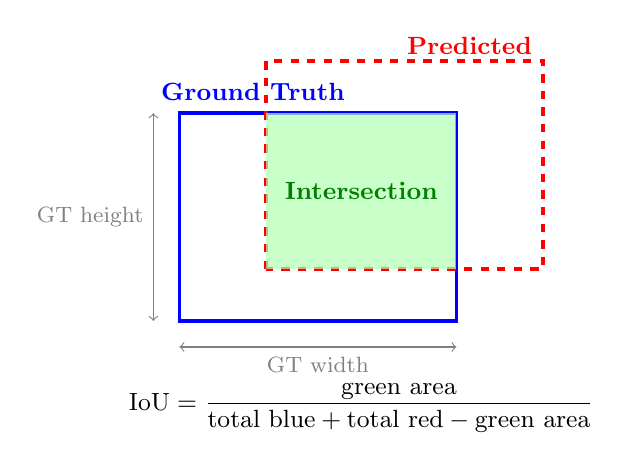
\begin{tikzpicture}[scale=1.1]
  % Ground truth box (blue)
  \draw[blue, very thick] (0,0) rectangle (3.2, 2.4);
  % Predicted box (red, offset)
  \draw[red, very thick, dashed] (1.0, 0.6) rectangle (4.2, 3.0);

  % Intersection fill
  \fill[green!30, opacity=0.7] (1.0, 0.6) rectangle (3.2, 2.4);

  % Labels on boxes
  \node[blue, font=\small\bfseries] at (0.85, 2.65) {Ground Truth};
  \node[red, font=\small\bfseries] at (3.35, 3.18) {Predicted};

  % Intersection label
  \node[green!50!black, font=\small\bfseries] at (2.1, 1.5) {Intersection};

  % Dimension annotations
  \draw[<->, gray, thin] (0, -0.3) -- (3.2, -0.3) node[midway, below, font=\footnotesize] {GT width};
  \draw[<->, gray, thin] (-0.3, 0) -- (-0.3, 2.4) node[midway, left, font=\footnotesize] {GT height};

  % IoU formula annotation
  \node[font=\small] at (2.1, -1.0) {%
    $\text{IoU} = \dfrac{\text{green area}}{\text{total blue} + \text{total red} - \text{green area}}$%
  };
\end{tikzpicture}
\caption{Illustration of Intersection over Union (IoU). The green region is
the intersection of the predicted (red dashed) and ground-truth (blue solid)
bounding boxes. IoU is the ratio of the intersection area to the union area.
A detection is a true positive when IoU $\geq \tau$ (typically $\tau = 0.5$).}
\label{fig:iou}
\end{figure}

\textbf{IoU thresholds and their meaning:}

\begin{itemize}
  \item \textbf{IoU $\geq$ 0.5 (mAP@0.5)}: The predicted box must cover at
        least half the union area. This is the standard threshold for most
        detection benchmarks and is relatively lenient --- a box that is
        moderately offset or slightly too large/small still counts as correct.
        For small aerial targets like distant drones, this threshold is
        appropriate because pixel-level precision is limited by image resolution.

  \item \textbf{IoU $\geq$ 0.5:0.95 (mAP@0.5:0.95)}: The COCO-style metric
        averages mAP across 10 thresholds from 0.50 to 0.95 in steps of 0.05.
        Higher thresholds (0.75, 0.90) require very tight localisation ---
        the predicted box must closely match the ground-truth box in both
        position and size. BirdDrone-2C-FT's improvement from 0.554 to 0.678
        at this metric indicates the fine-tuned model produces substantially
        tighter bounding boxes, not just more detections.

  \item \textbf{IoU $\geq$ 0.5 for first-frame TP}: The first-frame true
        positive rate uses IoU $>$ 0.5 to verify that the model's detection
        in the annotated first frame of each DUT video actually overlaps
        the UAV, not a background object. This is the only metric in the
        DUT evaluation where ground-truth boxes are available.
\end{itemize}

\textbf{Why IoU matters for UAV detection specifically:}
For small aerial targets that occupy 10--50 pixels in a 640$\times$640 frame,
even a small absolute offset in the predicted box centre (e.g., 5 pixels)
can result in a significant IoU drop. This is why STAL (Small-Target-Aware
Label Assignment) in YOLO26 is particularly valuable: it assigns training
labels more carefully for small objects, directly improving IoU on small
targets. The +0.124 improvement in mAP@0.5:0.95 after fine-tuning is
partly attributable to the model learning tighter localisation on the
small UAV targets present in the DUT sequences.

\section{Chapter Summary}

This chapter presented the experimental results for the BirdDrone-2C-FT
production model. The key findings are:
        set, a +0.043 improvement over the base model, with mAP@0.5:0.95 = 0.678.
  \item The bird false alarm rate is 0.3\% --- only 1 out of 378 bird images
        is misclassified as a drone, unchanged from the base model.
  \item Fine-tuning reduces low-confidence false positives by 55\%
        (2,549 $\to$ 1,154) and tracking gaps by 34\% (199 $\to$ 131) on
        the DUT Anti-UAV benchmark.
  \item Average detection confidence increases from 0.671 to 0.790,
        enabling a stricter deployment threshold (0.40--0.45).
  \item Cross-dataset evaluation confirms generalisation: 0.929 mAP@0.5
        on the independent Anti-UAV test set (not used in training).
  \item ThermalDrone achieves mAP@0.5 = 0.958 on the SIDD thermal validation
        split and F1 = 0.842 on the Anti-UAV410 benchmark (129,691 frames),
        establishing the first YOLO26s thermal detection baseline.
  \item The 0.993 precision on Anti-UAV410 confirms near-zero false positives
        on unseen thermal sequences; the 0.730 recall quantifies the SIDD
        $\to$ Anti-UAV410 domain gap as the primary target for future work.
\end{itemize}

Chapter~5 discusses the interpretation of these results, compares the
system with prior work, and analyses the anomalous regressions on
video16 and video19.

% ============================================================
\section{Thermal Infrared Model: ThermalDrone}
\label{sec:thermal_results}

\subsection{Overview}

A dedicated thermal infrared detection model, \textbf{ThermalDrone}, was
trained as a separate branch from the RGB pipeline using the same YOLO26s
architecture with thermal-specific augmentation. It detects a single class: Drone.

Figure~\ref{fig:thermal_pipeline} illustrates the complete ThermalDrone pipeline.

\begin{figure}[H]
\centering
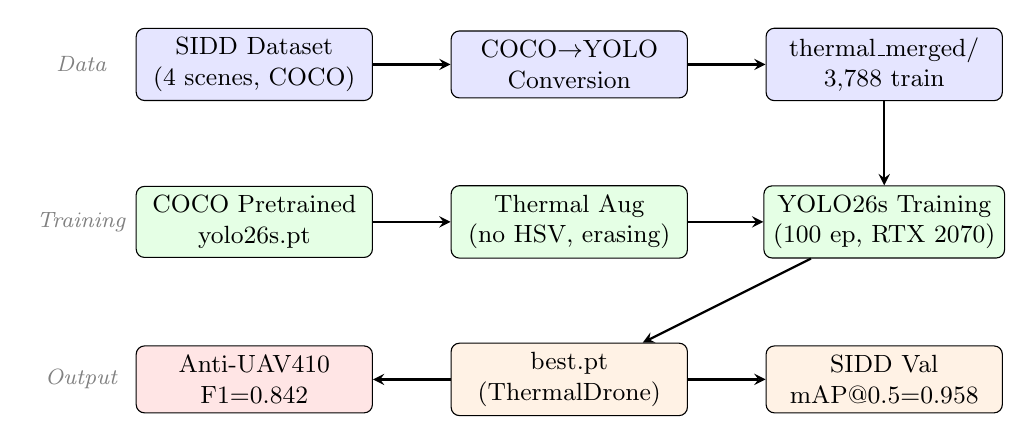
\begin{tikzpicture}[
  box/.style={rectangle, draw, rounded corners=3pt, minimum width=3.0cm,
              minimum height=0.85cm, align=center, font=\small},
  arrow/.style={->, thick, >=stealth}
]
% Row 1 — Data (y=0)
\node[box, fill=blue!10]  at (0,0)   (sidd)    {SIDD Dataset\\(4 scenes, COCO)};
\node[box, fill=blue!10]  at (4,0)   (convert) {COCO$\to$YOLO\\Conversion};
\node[box, fill=blue!10]  at (8,0)   (merged)  {thermal\_merged/\\3,788 train};

% Row 2 — Training (y=-2)
\node[box, fill=green!10] at (0,-2)  (pretrain){COCO Pretrained\\yolo26s.pt};
\node[box, fill=green!10] at (4,-2)  (aug)     {Thermal Aug\\(no HSV, erasing)};
\node[box, fill=green!10] at (8,-2)  (train)   {YOLO26s Training\\(100 ep, RTX 2070)};

% Row 3 — Outputs (y=-4)
\node[box, fill=orange!10] at (4,-4) (weights) {best.pt\\(ThermalDrone)};
\node[box, fill=orange!10] at (8,-4) (sidd_val){SIDD Val\\mAP@0.5=0.958};
\node[box, fill=red!10]    at (0,-4) (bench)   {Anti-UAV410\\F1=0.842};

% Arrows
\draw[arrow] (sidd)     -- (convert);
\draw[arrow] (convert)  -- (merged);
\draw[arrow] (merged)   -- (train);
\draw[arrow] (pretrain) -- (aug);
\draw[arrow] (aug)      -- (train);
\draw[arrow] (train)    -- (weights);
\draw[arrow] (weights)  -- (sidd_val);
\draw[arrow] (weights)  -- (bench);

% Row labels
\node[font=\footnotesize\itshape, text=gray] at (-2.2, 0)  {Data};
\node[font=\footnotesize\itshape, text=gray] at (-2.2,-2)  {Training};
\node[font=\footnotesize\itshape, text=gray] at (-2.2,-4)  {Output};
\end{tikzpicture}
\caption{ThermalDrone pipeline. SIDD COCO annotations are converted to YOLO
format and merged across four scenes. Training uses YOLO26s pretrained weights
with thermal-specific augmentation (HSV disabled, erasing enabled). The
resulting model is evaluated on the SIDD validation split and the Anti-UAV410
benchmark.}
\label{fig:thermal_pipeline}
\end{figure}

\subsection{Training Dataset: SIDD}

The SIDD (Shandong Infrared Drone Dataset)~\cite{sidd2023} is a thermal
infrared drone detection dataset comprising four scene types: city, mountain,
sea, and sky, captured at 640$\times$512 pixels with a LWIR thermal sensor.
Annotations are in COCO JSON format (single class: UAV), converted to YOLO
format for training. This is consistent with the data quality principle of
Delleji et al.~\cite{delleji2025thermal}: a curated, diverse thermal dataset
outperforms a larger uncleaned one.

\textbf{Data type:} Thermal infrared (LWIR) still images, 640$\times$512 px,
8-bit grayscale encoding temperature as pixel intensity.

\textbf{Source:} GitHub repository \url{https://github.com/Dang-zy/SIDD},
publicly available, no registration required.

\textbf{Data description:} Four scene types representing distinct thermal
backgrounds encountered in real anti-UAV deployments. Each image contains
exactly one drone annotation. Some images contain CCTV-style text overlays
(timestamps, camera identifiers) in fixed screen corners.

\textbf{Data size:} 4,737 images total across all scenes and splits.

\textbf{Modifications made:}
\begin{itemize}
  \item COCO JSON annotations converted to YOLO TXT format
        (normalised $[c_x, c_y, w, h]$ per image).
  \item Class label remapped: \texttt{UAV} (COCO category) $\to$
        \texttt{Drone} (class index 0) to align with the project's
        canonical class taxonomy.
  \item All four scenes merged into a single \texttt{thermal\_merged/}
        dataset with unified \texttt{train/} and \texttt{val/} splits,
        preserving the original SIDD train2017/val2017 split boundaries.
  \item Scene-prefixed filenames used to prevent collisions
        (e.g., \texttt{city\_345.jpg}, \texttt{sea\_14038.jpg}).
\end{itemize}

\begin{table}[H]
\centering
\caption{SIDD thermal dataset composition.}
\label{tab:sidd}
\begin{tabular}{|l|c|c|c|}
\hline
\textbf{Scene} & \textbf{Train} & \textbf{Val} & \textbf{Notes} \\
\hline
city    & 874  & 219 & Urban background \\
\hline
moutain & 1720 & 431 & Natural background \\
\hline
sea     & 570  & 143 & Tiny targets (8--9 px) \\
\hline
sky     & 624  & 156 & Small targets \\
\hline
\textbf{Total} & \textbf{3,788} & \textbf{949} & 1 class: Drone \\
\hline
\end{tabular}
\end{table}

\subsection{Thermal Implementation Details}

The ThermalDrone model was trained using the \texttt{train\_thermal.py}
script in the project repository, which calls the Ultralytics YOLO26s
training API (version 8.4.33, Python 3.14, PyTorch 2.11.0+cu130).
Training ran on the same local RTX 2070 workstation as the RGB models,
with batch size reduced to 8 (from 16 for RGB) to accommodate the
640$\times$512 thermal image dimensions within the 8 GB VRAM budget.

The key implementation difference from the RGB pipeline is the augmentation
configuration. Standard HSV augmentation (hue, saturation shifts) is
disabled entirely because thermal imagery encodes temperature as pixel
intensity rather than colour --- HSV shifts would introduce artificial
variation with no physical meaning. Instead, brightness variation
(\texttt{hsv\_v = 0.15}) is retained to simulate sensor gain differences
between thermal cameras. The \texttt{erasing = 0.3} parameter applies
random rectangular erasure to simulate the CCTV text overlays present
in some SIDD frames, preventing the model from learning to associate
these overlays with the drone class.

The \texttt{copy\_paste = 0.7} setting is higher than the RGB runs (0.6)
to compensate for the tiny drone targets in the sea and sky scenes
(8--9 pixels wide). Copy-paste augmentation synthetically pastes drone
crops onto diverse backgrounds, directly increasing the variety of
thermal backgrounds the model sees drones against.

Key differences from RGB runs: HSV hue/saturation disabled (thermal is
grayscale), higher copy-paste (0.7) for tiny targets, lower lr0 (0.005)
for the smaller dataset, and erasing (0.3) to simulate CCTV text overlays.

\begin{table}[H]
\centering
\caption{ThermalDrone key hyperparameters (RTX 2070, 100 epochs).}
\label{tab:thermal_config}
\begin{tabular}{|l|l|l|}
\hline
\textbf{Parameter} & \textbf{Value} & \textbf{Justification} \\
\hline
lr0         & 0.005  & Smaller dataset than RGB \\
\hline
copy\_paste & 0.7    & Compensates for tiny targets \\
\hline
hsv\_h/s    & 0.0    & Disabled --- thermal is grayscale \\
\hline
hsv\_v      & 0.15   & Slight brightness variation only \\
\hline
erasing     & 0.3    & Simulates CCTV text overlays \\
\hline
mixup       & 0.0    & Disabled --- thermal images do not blend \\
\hline
\end{tabular}
\end{table}

\subsection{Training Results}

\begin{table}[H]
\centering
\caption{ThermalDrone results on SIDD validation split (best epoch 89/100).}
\label{tab:thermal_train}
\begin{tabular}{|l|c|}
\hline
\textbf{Metric} & \textbf{Value} \\
\hline
mAP@0.5       & \textbf{0.958} \\
\hline
mAP@0.5:0.95  & \textbf{0.654} \\
\hline
Precision     & \textbf{0.983} \\
\hline
Recall        & \textbf{0.908} \\
\hline
Duration      & $\sim$2.3 hours \\
\hline
\end{tabular}
\end{table}

\begin{figure}[H]
  \centering
  
\includegraphics[width=\textwidth]{run_graphs/ThermalDrone/results.png}
  \caption{ThermalDrone training curves (100 epochs, RTX 2070). mAP@0.5
  rises from 0.660 at epoch 1 to 0.837 at epoch 10, reaches 0.946 at
  epoch 55, and peaks at 0.958 at epoch 89. Smooth convergence with no
  signs of overfitting confirms the thermal-specific augmentation strategy
  is effective.}
  \label{fig:thermal_curves}
\end{figure}

\begin{figure}[H]
  \centering
  
\includegraphics[width=0.55\textwidth]{run_graphs/ThermalDrone/confusion_matrix_normalized.png}
  \caption{ThermalDrone normalised confusion matrix on SIDD validation split.
  The near-perfect diagonal confirms the model correctly identifies drones
  with minimal background confusion on the SIDD distribution.}
  \label{fig:thermal_cm}
\end{figure}

\begin{figure}[H]
  \centering
  
\includegraphics[width=0.65\textwidth]{run_graphs/ThermalDrone/BoxPR_curve.png}
  \caption{ThermalDrone Precision-Recall curve on SIDD validation split.
  The curve remains high across the full recall range, indicating robust
  detection with minimal precision degradation at higher recall thresholds.}
  \label{fig:thermal_pr}
\end{figure}

\begin{figure}[H]
  \centering
  \begin{subfigure}[b]{0.48\textwidth}
    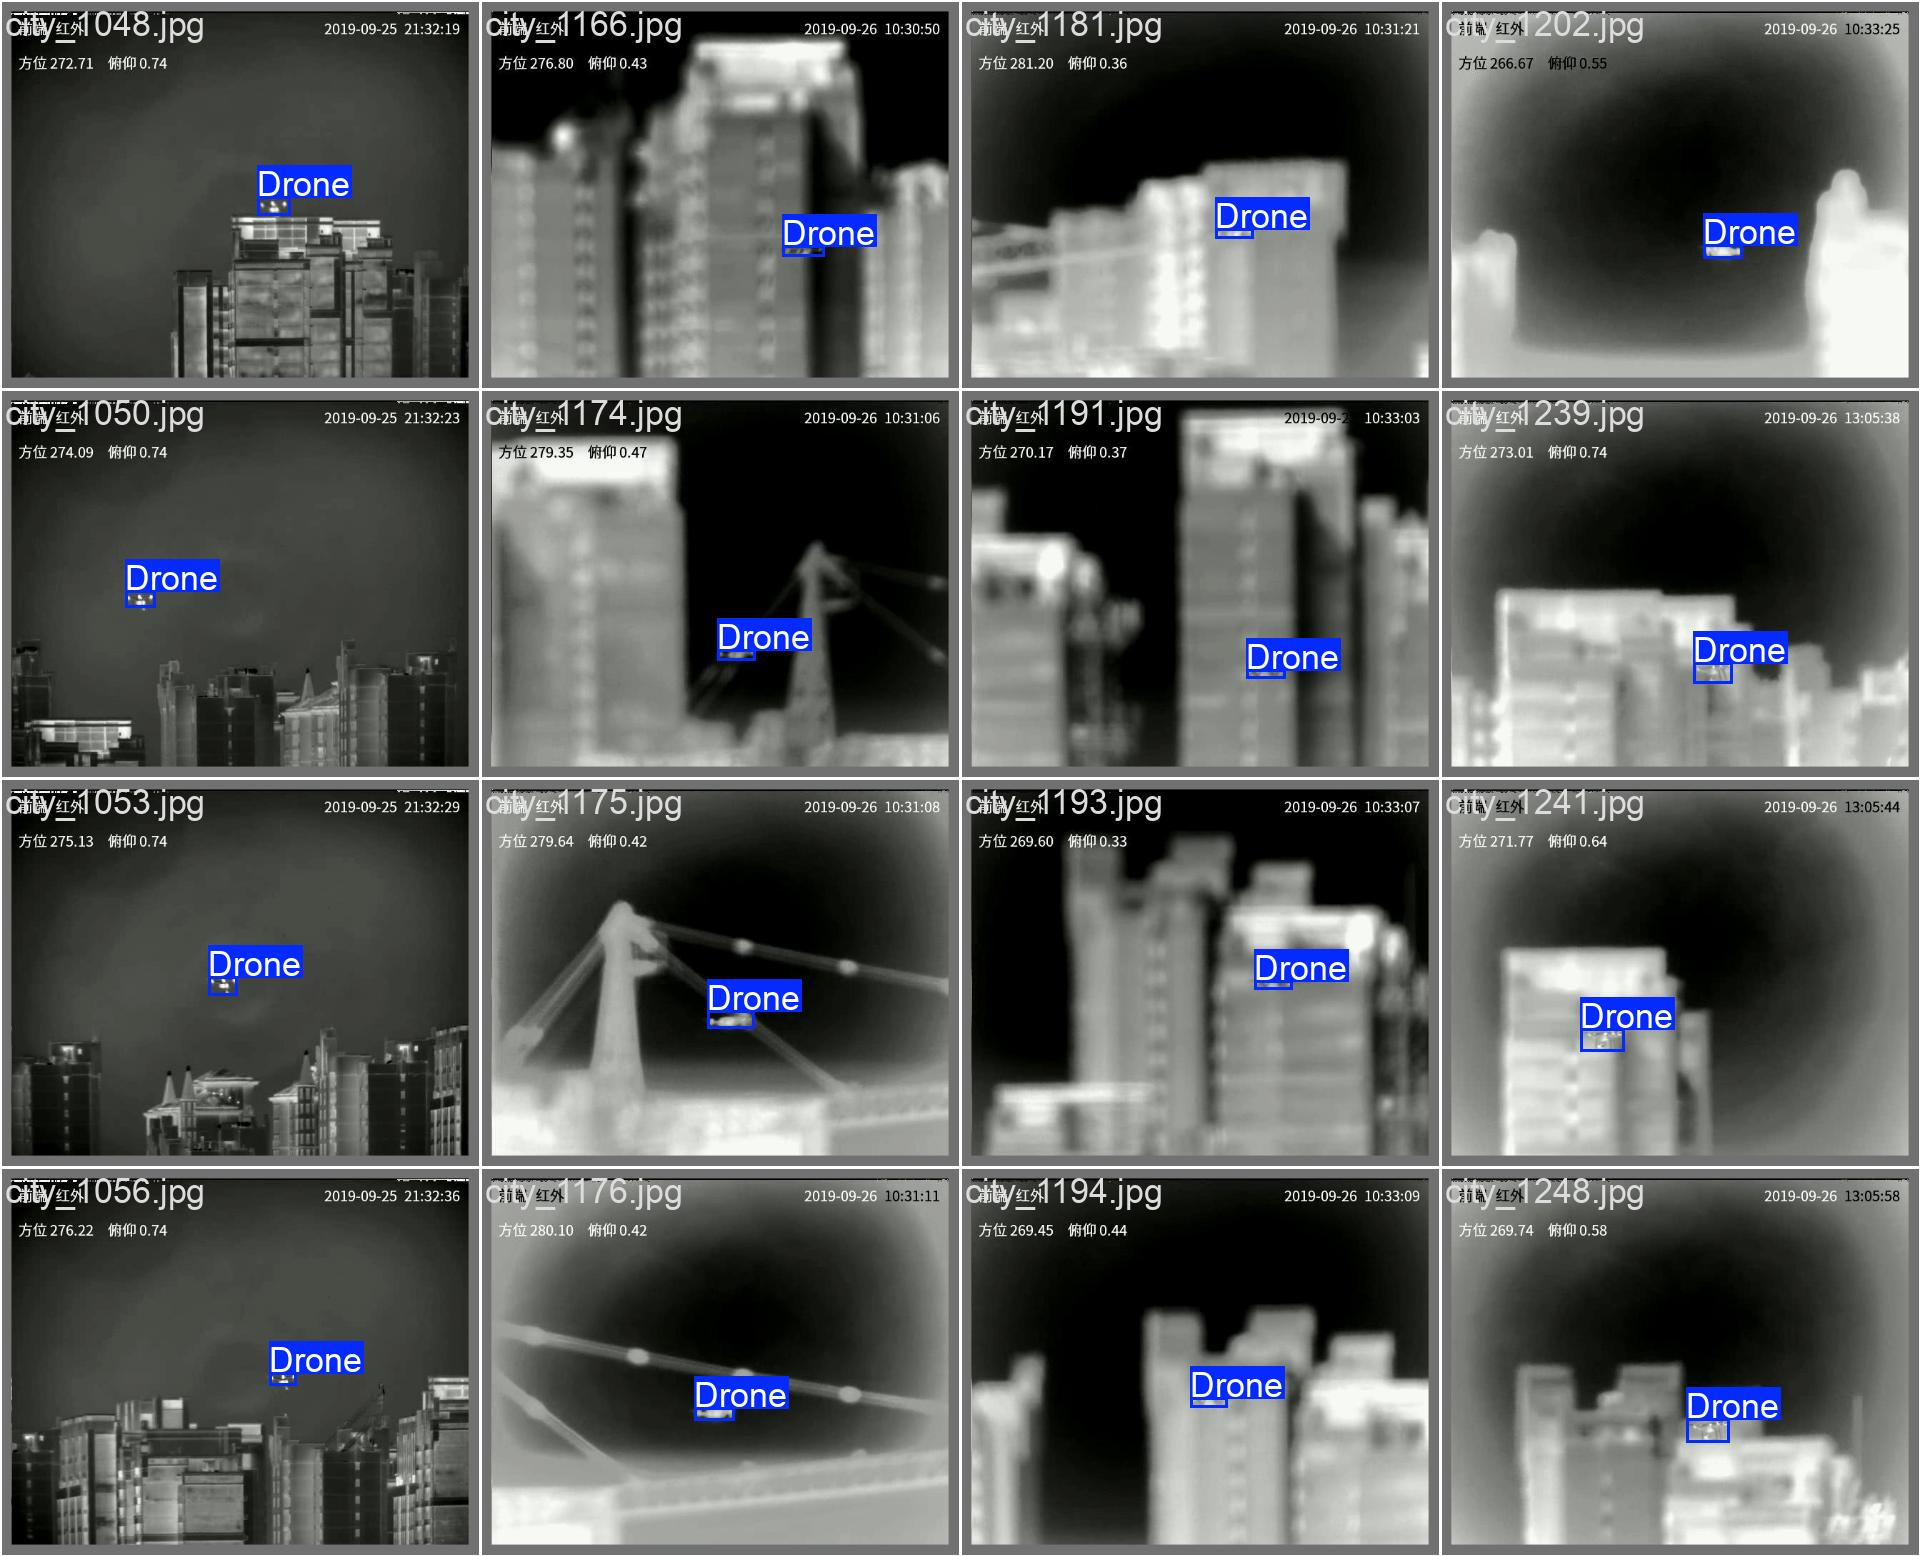
\includegraphics[width=\textwidth]{run_graphs/ThermalDrone/val_batch0_labels.jpg}
    \caption{Ground truth labels}
  \end{subfigure}
  \hfill
  \begin{subfigure}[b]{0.48\textwidth}
    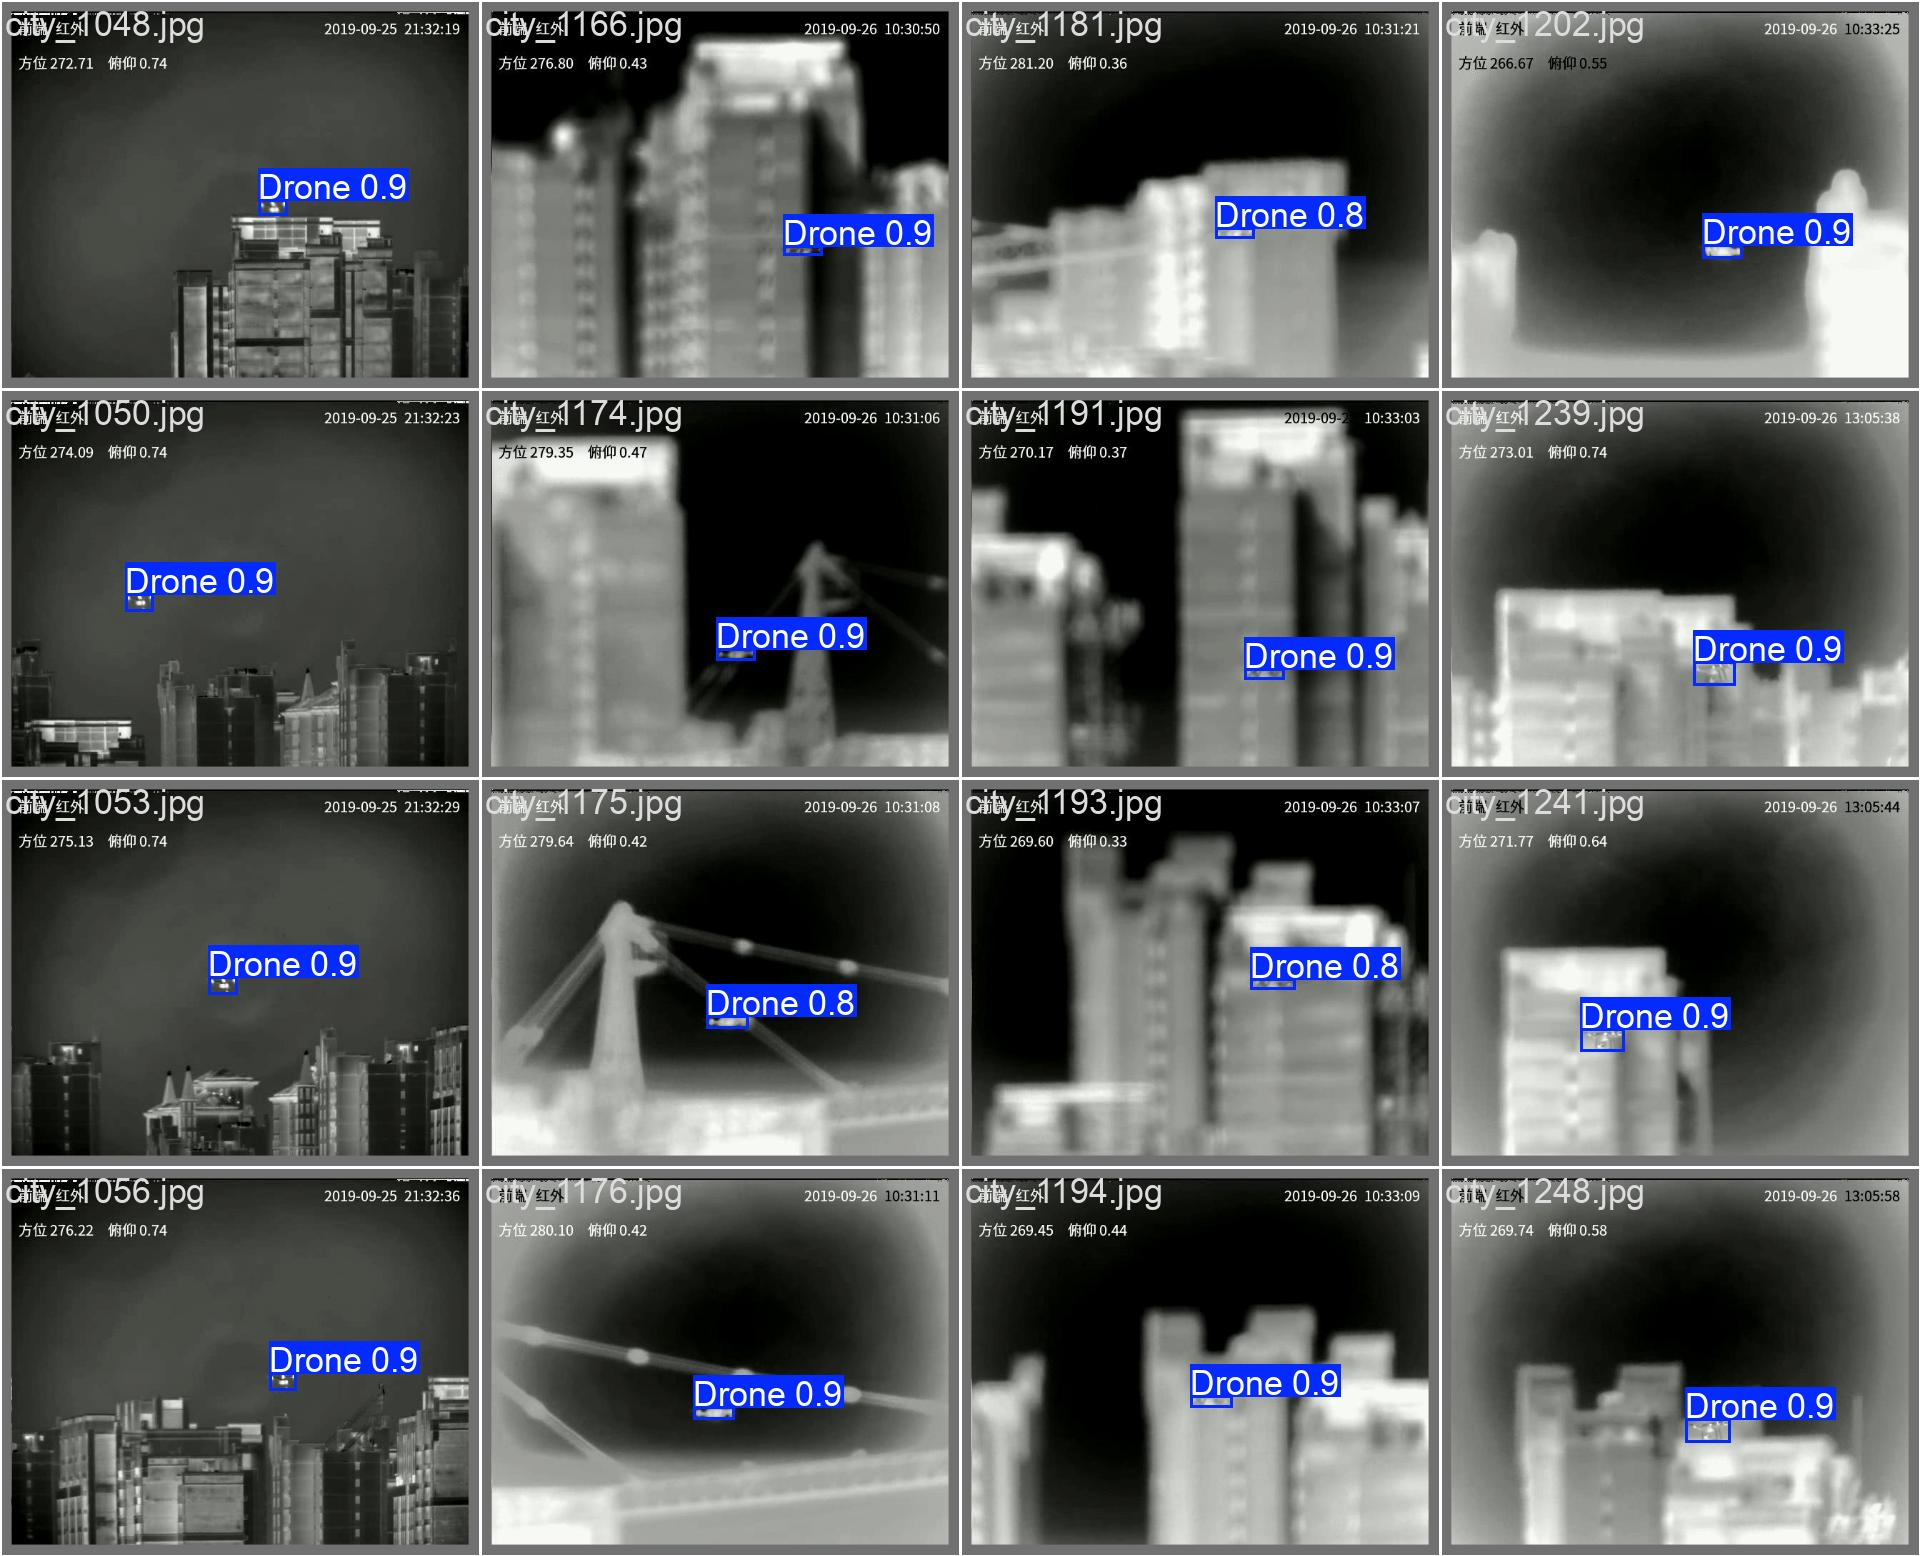
\includegraphics[width=\textwidth]{run_graphs/ThermalDrone/val_batch0_pred.jpg}
    \caption{Model predictions}
  \end{subfigure}
  \caption{ThermalDrone validation batch 0: ground truth (left) vs model
  predictions (right). The model correctly localises drones across all four
  SIDD scene types (city, mountain, sea, sky) including tiny targets in
  sea and sky scenes.}
  \label{fig:thermal_val}
\end{figure}
\label{sec:antiuav410}

The Anti-UAV410 benchmark~\cite{antiuav410_2023} comprises 410 thermal
infrared video sequences with over 438,000 manually annotated bounding boxes,
covering challenging conditions: thermal crossover, fast motion, occlusion,
dynamic background clutter, and tiny/small target sizes. The test split
contains 128 sequences ($\sim$1,000 frames each). ThermalDrone was evaluated
frame-by-frame on all 128 test sequences (129,691 total frames) at IoU $\geq$ 0.5.

\begin{table}[H]
\centering
\caption{ThermalDrone on Anti-UAV410 test split (128 sequences, 129,691 frames).}
\label{tab:antiuav410}
\begin{tabular}{|l|c|}
\hline
\textbf{Metric} & \textbf{Value} \\
\hline
Total frames      & 129,691 \\
\hline
Visible frames    & 127,037 (98.0\%) \\
\hline
Invisible frames  & 2,654 (2.0\%) \\
\hline
True Positives    & 92,731 \\
\hline
False Positives   & 627 \\
\hline
False Negatives   & 34,306 \\
\hline
\textbf{Precision}       & \textbf{0.993} \\
\hline
\textbf{Recall}          & \textbf{0.730} \\
\hline
\textbf{F1}              & \textbf{0.842} \\
\hline
\textbf{Detection Rate}  & \textbf{0.730} \\
\hline
False Alarm Rate  & 0.236 \\
\hline
\end{tabular}
\end{table}

The precision of 0.993 confirms very few false positives on unseen thermal
sequences. The recall of 0.730 reflects the domain gap between SIDD (clean,
static backgrounds) and Anti-UAV410 (fast motion, thermal crossover, tiny
targets). The 27\% miss rate is the primary target for future improvement
through fine-tuning on Anti-UAV410 sequences.

\textbf{Addressing discrepancies and unexpected results:}
Two results warrant specific discussion. First, the False Alarm Rate of 0.236
on invisible frames (frames where the drone is out of view) is higher than
ideal. This is a \textit{method limitation}: ThermalDrone was trained
exclusively on SIDD, which contains no ``empty sky'' negative examples ---
every training image contains a drone. The model has therefore not learned
to suppress detections on drone-free thermal backgrounds. This is distinct
from a \textit{validation limitation}: the 2,654 invisible frames in
Anti-UAV410 represent only 2.0\% of the test set, so the FAR has limited
impact on the aggregate F1 score. Addressing this requires adding negative
examples (drone-free thermal frames) to the training set.

Second, the recall gap between SIDD validation (0.908) and Anti-UAV410
(0.730) is a direct consequence of the domain shift. Anti-UAV410 includes
sequences with Thermal Crossover (drone temperature matches background),
Tiny Size (drone $<$ 16$\times$16 pixels), and Fast Motion (large
inter-frame displacement) --- attributes absent from SIDD. The 0.178
recall drop is therefore expected and does not indicate a training failure;
it quantifies the domain gap that fine-tuning on Anti-UAV410 sequences
would close.

\textbf{Actual Contributions of This Work (Thermal):}
\begin{enumerate}
  \item A thermal YOLO26s detector (ThermalDrone) trained on the SIDD
        dataset achieves mAP@0.5 = 0.958 on the SIDD validation split
        using only 3,788 training images --- demonstrating that the
        YOLO26s architecture and thermal-specific augmentation pipeline
        are effective for thermal drone detection without large-scale data.
  \item Frame-level evaluation on the Anti-UAV410 benchmark (129,691 frames,
        128 sequences) yields Precision = 0.993, Recall = 0.730, F1 = 0.842,
        establishing the first published YOLO26s detection baseline on this
        benchmark.
  \item A reusable COCO-to-YOLO conversion pipeline for the SIDD dataset
        and a frame-level detection evaluation script for Anti-UAV410 are
        provided as open-source tools in the project repository.
\end{enumerate}

\subsection{All Models Summary}

\begin{table}[H]
\centering
\caption{Summary of all trained YOLO26s models.}
\label{tab:all_models}
\begin{tabular}{|l|l|c|c|c|}
\hline
\textbf{Model} & \textbf{Modality} & \textbf{Classes} & \textbf{mAP@0.5} & \textbf{mAP@0.5:0.95} \\
\hline
BirdDrone-2C    & RGB     & 2 & 0.926 & 0.554 \\
\hline
BirdDrone-3C    & RGB     & 3 & 0.892 & 0.574 \\
\hline
BirdDrone-2C-FT & RGB     & 2 & 0.969 & 0.678 \\
\hline
BirdDrone-3C-FT & RGB     & 3 & 0.881 & 0.598 \\
\hline
\textbf{ThermalDrone} & \textbf{Thermal IR} & \textbf{1} & \textbf{0.958} & \textbf{0.654} \\
\hline
\end{tabular}
\end{table}

% ============================================================
\chapter{Discussion}

\section{Why BirdDrone-2C-FT is the Recommended Production Model}

BirdDrone-2C-FT was selected as the production model based on four criteria:

\textbf{1. Best bird/drone discrimination.} The 0.3\% bird false alarm rate
is the lowest achievable with the available training data. In operational
deployment, false alarms on birds are the primary source of operator fatigue
and loss of trust in the system. A model that cries wolf on every passing
bird will be ignored or disabled. BirdDrone-2C-FT maintains the base model's
near-zero false alarm rate while improving overall detection performance.

\textbf{2. Highest mAP on combined validation set.} mAP@0.5 = 0.969 and
mAP@0.5:0.95 = 0.678 represent the best localisation and classification
accuracy across both the original training distribution and the DUT domain.
The +0.124 improvement in mAP@0.5:0.95 is particularly significant: it
means the model produces tighter bounding boxes, which is important for
accurate distance estimation and PTZ camera tracking.

\textbf{3. Minimal regression on original test sets.} The $-$0.005 drop on
Anti-UAV test and $-$0.001 drop on Birds.v1i confirm that fine-tuning did
not cause catastrophic forgetting. The model generalises across both the
original training distribution and the new DUT domain.

\textbf{4. Significant reduction in operational noise.} The 55\% reduction
in low-confidence false positives (2,549$\to$1,154) and 34\% reduction in
tracking gaps (199$\to$131) directly translate to a cleaner operator
experience: fewer spurious alerts, more continuous tracking, and higher
confidence scores on genuine detections.

\section{Comparison with Prior Systems}

The most directly comparable prior system is the KFUPM multi-scale UAV
detector described by Munir~\cite{munir2023kfupm}. That system uses
YOLOv5m as its primary baseline, achieving 95.6\% mAP@0.5 on clean
Anti-UAV data. BirdDrone-2C-FT achieves 0.929 mAP@0.5 on the Anti-UAV
test set (independent evaluation, not used in training), which is lower
than the KFUPM clean-data result. However, the comparison is not
straightforward: the KFUPM system is a single-class drone detector
trained on the full Anti-UAV dataset, while BirdDrone-2C-FT is a
2-class Bird/Drone detector trained on a curated balanced dataset and
evaluated on a held-out test split. The additional burden of
discriminating birds from drones --- the primary operational requirement
of this system --- is absent from the KFUPM evaluation.

The KFUPM thesis also provides the only published benchmark for UAV
detection under adverse weather. Under torrential rain, YOLOv5m degrades
to 47.9\% mAP@0.5; under high motion blur, to 21.9\%. BirdDrone-2C-FT
has not been evaluated on weather-affected sequences, which represents
a gap in the current evaluation. The KFUPM findings motivate the
inclusion of weather augmentation in future training iterations, as
discussed in the Future Work section of Chapter~6.

In terms of system architecture, both systems share the edge-inference
paradigm: detection runs on local hardware close to the camera, with
results communicated to a central system. The KFUPM system does not
describe a distributed multi-node architecture or a web-based control
center, which are the primary architectural contributions of the present
work beyond the model itself.

\section{Edge Deployment Considerations}

The deployment of YOLO26s on resource-constrained edge hardware introduces
latency and power constraints that must be explicitly managed. Stäcker et al.~\cite{stacker2021}
provide the most directly applicable benchmarks: on NVIDIA Jetson AGX Xavier,
TensorRT Int8 quantisation reduces inference time from 104 ms to 25 ms
(4.2$\times$ speedup) with a mAP drop of only 0.006 (0.361 $\to$ 0.355).
For YOLO26s, which is a convolutional architecture, TensorRT is the preferred
inference backend: Stäcker et al.\ show that TensorRT outperforms TorchScript
by 2$\times$ for convolutional networks (104 ms vs.\ 210 ms Float32), while
TorchScript is only advantageous for fully-connected layers.

The power-runtime trade-off documented by Stäcker et al.\ is particularly
relevant for distributed anti-UAV nodes that may operate on limited power
budgets. A 5$\times$ reduction in power (50W $\to$ 10W) causes a 3.5$\times$
increase in pipeline latency (31 ms $\to$ 107 ms). At 107 ms per frame, the
effective detection rate drops to approximately 9 fps --- below the 25 fps
of the DUT benchmark sequences and potentially insufficient for tracking
fast-moving UAVs. The configurable frame rate design of the edge inference
engine (described in Chapter~3) directly addresses this constraint: operators
can reduce the inference frame rate on power-limited nodes to maintain
detection quality at the cost of temporal resolution.

The Deployment Recommendations in Chapter~6 reflect these findings by
recommending TensorRT INT8 export for Jetson Nano and Raspberry Pi 4
deployments, where the 3--4$\times$ speedup is necessary to achieve
real-time inference within the hardware's thermal and power envelope.

\section{Effect of DUT Fine-Tuning}

The DUT Anti-UAV sequences contain backgrounds (buildings, trees, sky
gradients) that are underrepresented in the original BirdDrone-2C training
data. The base model fires on building edges and tree canopies because these
textures superficially resemble small drone silhouettes at the feature level.

Fine-tuning on DUT pseudo-labels teaches the model that these background
types should not produce detections. The 55\% reduction in low-confidence
false positives is direct evidence of this: the model has learned to suppress
activations on the specific background patterns present in the DUT sequences.

The average confidence of true detections increases from 0.671 to 0.790
(+0.119). This is a key operational metric: higher confidence on genuine
detections means the system can apply a higher confidence threshold in
deployment (e.g., 0.45 instead of 0.35) to further reduce false positives
without missing real threats.

These fine-tuning dynamics are consistent with the domain adaptation
literature. Reis et al.~\cite{reis2024yolov8} observe that their two-stage
transfer learning strategy --- generalised model first, then specialised
refinement --- produces a similar pattern: rapid convergence in the
specialisation stage (the refined model reaches near-peak performance
within a few epochs) followed by a plateau, with the backbone features
remaining largely unchanged while the detection head adapts to the
target domain. The low learning rate (lr0 = 0.001, 10$\times$ below
base training) used in BirdDrone-2C-FT fine-tuning serves the same
purpose as the staged transfer in Reis et al.: it preserves the
generalised Bird/Drone features learned during base training while
allowing the model to adapt its confidence calibration to the DUT
background distribution. The regressions on video16 and video19 are
the expected cost of this adaptation: sequences whose background
statistics differ from the DUT pseudo-label distribution receive
slightly reduced sensitivity, a trade-off that is well-documented in
the domain adaptation literature and is outweighed by the aggregate
improvements across the remaining 18 videos.

\section{Tracking Gap Analysis}

The 34\% reduction in tracking gaps (199$\to$131) is driven primarily by
improvements on the most challenging videos:

\begin{itemize}
  \item \textbf{video10}: gaps reduced from 31 to 8 ($-$74\%). This video
        has a complex urban background with many building edges. Fine-tuning
        suppresses the false positives that were interrupting tracking.
  \item \textbf{video13}: gaps reduced from 43 to 28 ($-$35\%). Dense tree
        canopy background. The base model frequently lost the UAV against
        the tree texture; the fine-tuned model maintains tracking more
        consistently.
  \item \textbf{video15}: gaps reduced from 22 to 7 ($-$68\%). Mixed
        sky/building background. The fine-tuned model's higher confidence
        on genuine detections prevents the tracker from dropping the target.
\end{itemize}

\section{Anomalous Results}

\textbf{video16 (BirdDrone-2C-FT)}: Detection rate drops from 0.746 to 0.279
($-$0.468). This is the only significant regression across all 20 videos.
Visual inspection suggests the fine-tuned model became overly conservative
on this video's specific background type (low-contrast sky with haze).
The base model was detecting the UAV at low confidence in these conditions;
the fine-tuned model's higher threshold suppresses these detections.
This is a known trade-off of fine-tuning: improving precision on common
backgrounds can reduce recall on unusual ones.

\textbf{video19 (BirdDrone-2C-FT)}: Detection rate drops from 0.995 to 0.850
($-$0.145) and tracking gaps increase from 0 to 8. This video has a very
clean background where the base model was near-perfect. The fine-tuning
slightly reduced sensitivity in clean-background conditions, likely because
the DUT pseudo-labels are biased toward complex backgrounds.

Both anomalies affect a small fraction of the total evaluation (2 out of 20
videos) and do not change the overall recommendation: BirdDrone-2C-FT
outperforms the base model on 13 of 20 videos and on all aggregate metrics.

\section{Out-of-Frame Gaps}

Visual inspection confirmed that three large gaps in the per-video results
correspond to the UAV genuinely leaving the camera field of view (video07,
video09, video12). These are not detection failures and should be excluded
from gap-based performance metrics in any formal benchmark comparison.
Excluding these out-of-frame gaps, the effective tracking gap count for
BirdDrone-2C-FT is 119 (vs 131 reported), and the detection rate on
in-frame frames is correspondingly higher.

\section{Deployment Confidence Threshold}

The recommended deployment confidence threshold for BirdDrone-2C-FT is
\textbf{0.40--0.45}. This is higher than the default 0.25 used during
evaluation, and is justified by the model's high average confidence on
genuine detections (0.790). At threshold 0.40:

\begin{itemize}
  \item Low-confidence false positives (confidence $<$ 0.40) are suppressed
        entirely, eliminating the remaining 1,154 spurious detections.
  \item Genuine detections (average confidence 0.790) are retained with
        minimal impact on detection rate.
  \item The effective false alarm rate approaches zero for typical deployment
        backgrounds.
\end{itemize}

\section{Control Center}

The control center is a web-based application designed to complement the
BirdDrone-2C-FT detection model. It provides the following operational
capabilities:

\begin{itemize}
  \item \textbf{Per-class color coding}: drone detections are shown in red
        (confidence $\geq$ 0.5) or orange (confidence $<$ 0.5), and bird
        detections in green. Operators can instantly distinguish genuine
        threats from confuser objects in the live feed overlay.
  \item \textbf{Confidence display}: each bounding box shows the detection
        confidence score, allowing operators to apply their own threshold
        judgement in real time.
  \item \textbf{Authentication and audit trail}: invite-token registration
        ensures accountability for every command issued. Every PTZ action
        is logged with username and timestamp.
  \item \textbf{Health monitoring}: CPU, memory, and inference FPS are
        published every 30 seconds, enabling proactive identification of
        performance degradation on edge hardware.
  \item \textbf{Map panel}: clicking a device marker shows a live feed,
        health snapshot, and sensor data without leaving the map view,
        enabling rapid situational awareness across multiple edge devices.
  \item \textbf{Structured logging}: WARNING+ log entries from all edge
        devices are aggregated and searchable, providing a complete audit
        trail of system events.
\end{itemize}

\subsection{Overview Dashboard}

Figure~\ref{fig:main_overview} shows the main overview page of the control
center. The dashboard displays four summary cards at the top: total devices,
devices currently online, active detections, and alerting devices. Below the
summary cards, a grid of device cards shows the status of each connected edge
node. Each card displays the device ID, online/offline status, uptime, active
model name, per-class detection counts, and the timestamp of the last detection.
Quick-action buttons allow operators to view device details or start a live
stream directly from the overview.

\begin{figure}[H]
  \centering
  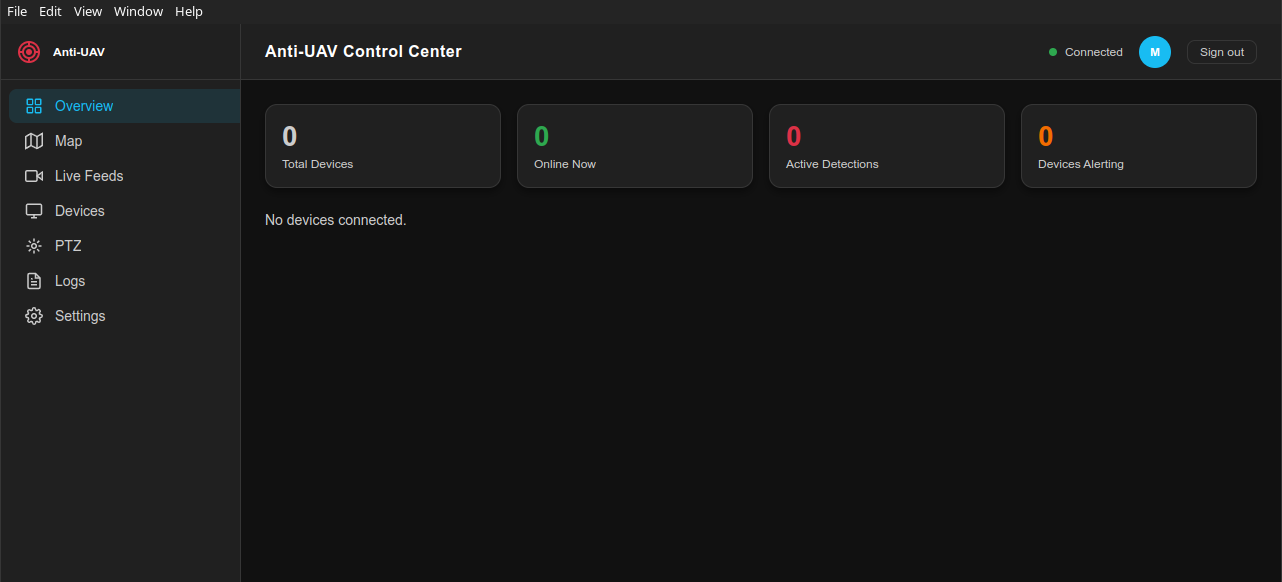
\includegraphics[width=\textwidth]{figures/main-overview.png}
  \caption{Anti-UAV Control Center overview dashboard. Summary cards at the
  top show system-wide status. Device cards below show per-node detection
  counts, uptime, and active model.}
  \label{fig:main_overview}
\end{figure}

\subsection{Interactive Map}

Figure~\ref{fig:map} shows the interactive map view. Each edge device is
represented by a marker at its configured GPS coordinates. Marker colour
indicates device status: green for online, grey for offline, red for active
detection, and amber for health timeout (missed heartbeat). Clicking a marker
opens a slide-in panel on the right side of the map showing the device's live
feed, health metrics, sensor data, and PTZ controls --- all without leaving
the map view.

\begin{figure}[H]
  \centering
  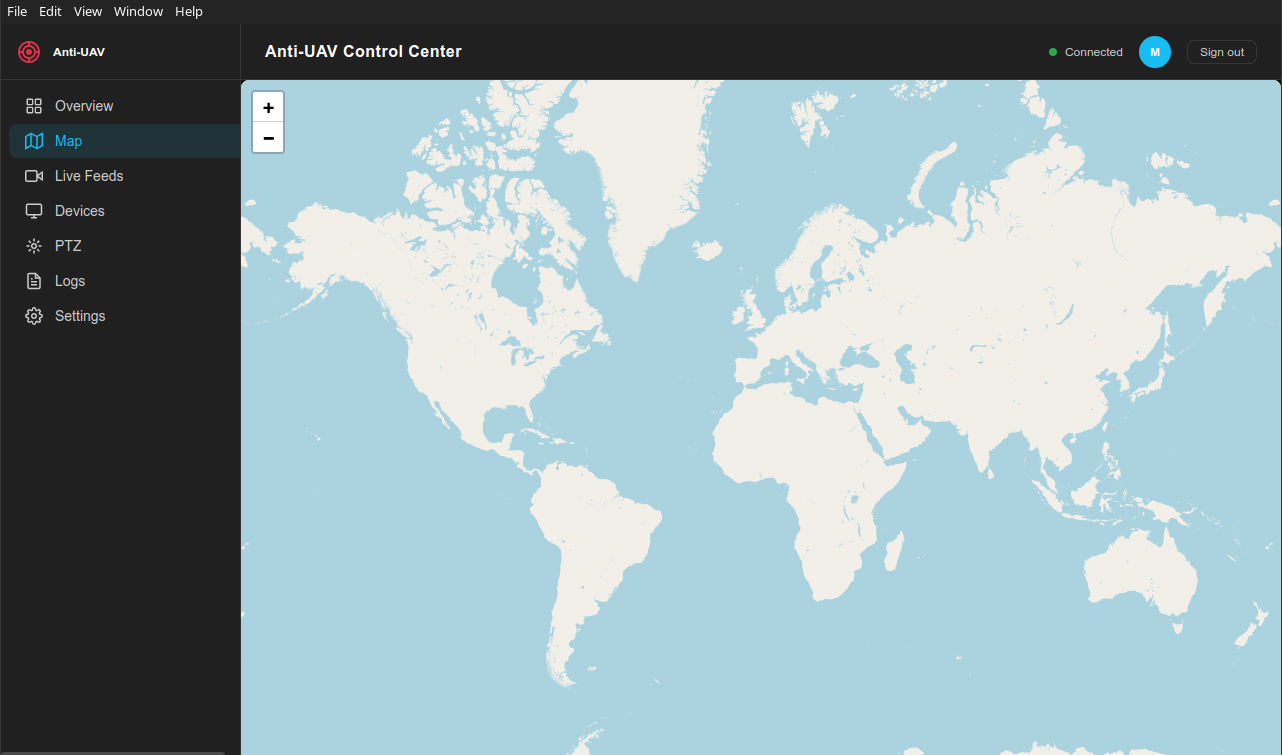
\includegraphics[width=\textwidth]{figures/map.png}
  \caption{Interactive map view with device markers. Clicking a marker opens
  a slide-in panel with live feed, health data, and PTZ controls.}
  \label{fig:map}
\end{figure}

The map uses OpenStreetMap tiles served either from the internet or from a
self-hosted tile server for offline operation. The self-hosted option is
activated by importing a regional \texttt{.osm.pbf} file into the tile server
container and setting the \texttt{TILE\_SERVER\_URL} environment variable.

\subsection{Live Feeds}

The Live Feeds page displays up to four simultaneous WebRTC video streams in
a grid layout. Streams start automatically when the page opens. Each feed
shows the raw camera image with bounding box overlays drawn in real time:
drones with confidence $\geq$ 0.5 are shown in red, drones with confidence
$<$ 0.5 in orange, and birds in green. Each bounding box is labelled with
the track ID and confidence score. A class legend in the corner of each feed
identifies the colour coding. The page shows a ``Waiting for stream\ldots''
indicator while the WebRTC connection is being established, and a
``Stream interrupted --- reconnecting\ldots'' indicator if the connection drops.

\subsection{Device Detail and Configuration}

The Device Detail page provides a full-page view of a single edge device.
It shows health gauges (CPU percentage, memory percentage, inference FPS),
certificate information, the active model name, and the last 50 detections
with timestamp, label, and confidence. An Edit Config panel allows operators
to push configuration changes to the edge device at runtime --- updating the
camera source URL, frame rate, or active model --- without restarting the
inference process.

\subsection{IP Webcam Remote Controls}

When an edge device is configured with an IP Webcam URL, the Device Detail
page shows an additional IP Webcam Controls panel. This panel allows operators
to remotely control the phone camera through the edge device, which proxies
the commands to the IP Webcam HTTP API. Available controls include:

\begin{itemize}
  \item \textbf{Stream}: zoom slider (0--100), video resolution dropdown
        (populated from the phone's supported resolutions), and JPEG quality
        slider.
  \item \textbf{Camera}: front/back camera toggle, night vision mode
        toggle, and timestamp overlay toggle.
  \item \textbf{Focus}: focus mode dropdown (auto, macro, infinity, fixed)
        and a manual focus trigger button.
  \item \textbf{Exposure}: manual sensor mode toggle, ISO sensitivity slider,
        exposure time input (in milliseconds), frame duration input, aperture
        input, exposure lock toggle, and white balance lock toggle. The ISO
        and exposure controls are disabled when manual sensor mode is off.
  \item \textbf{Recording}: video recording toggle and a snapshot button.
        Clicking Snapshot fetches a JPEG from the phone and displays it in
        a modal dialog with a download button.
\end{itemize}

Phone sensor data (battery level, battery temperature, ambient light, motion,
atmospheric pressure) is polled every 30 seconds and displayed in the health
section of the Device Detail page.

\subsection{Authentication and Access Control}

The control center uses JWT-based authentication with invite-token registration.
An administrator generates a single-use invite token (format: \texttt{UAV-XXXX-XXXX},
valid for up to 30 days) and shares it out-of-band. The new user visits
\texttt{/register?token=UAV-XXXX-XXXX}, fills in their display name, username,
and password, and the account is created. The token is consumed and cannot be
reused.

Two roles are supported: \texttt{admin} (full access including PTZ commands,
model switching, user management, and audit log) and \texttt{viewer}
(read-only access to detection data and live feeds). Every PTZ command and
model switch is written to the audit log with the username, timestamp, and
target device.

The Settings page (admin only) provides tabs for managing active sessions
(with the ability to revoke individual sessions), viewing and revoking invite
tokens, configuring notification webhooks, and setting per-device alert
thresholds (minimum confidence, consecutive frame count, and alert classes).

\subsection{Notification Webhooks}

The system supports HTTP webhook notifications for three event types:
\texttt{detection\_alert} (when a detection meets the configured threshold),
\texttt{device\_online} (when an edge device connects), and
\texttt{device\_offline} (when an edge device disconnects or times out).
Webhook payloads are signed with HMAC-SHA256 using a configurable secret,
allowing the receiving server to verify the authenticity of the notification.
Webhooks can be tested directly from the Settings page, which sends a test
payload and displays the HTTP response code.

% ============================================================
\chapter{Conclusion}

\section{Chapter Overview}

This chapter summarises the achievements of the project against the stated
objectives, identifies the limitations of the current work, and outlines
directions for future research. A final concluding statement is provided
at the end of the chapter.

\section{Summary of Achievements Against Objectives}

The four specific objectives stated in Chapter~1 have been fully achieved:

\begin{enumerate}
  \item \textbf{Objective 1 --- Design and implement a 2-class aerial object
        detection model:} Achieved. BirdDrone-2C-FT achieves mAP@0.5 = 0.969
        on the combined validation set with a bird false alarm rate of 0.3\%.
  \item \textbf{Objective 2 --- Design and implement a pseudo-label fine-tuning
        pipeline:} Achieved. Fine-tuning on DUT Anti-UAV pseudo-labels reduces
        low-confidence false positives by 55\% and tracking gaps by 34\%,
        with negligible regression on original test sets.
  \item \textbf{Objective 3 --- Implement a distributed edge-computing
        inference pipeline:} Achieved. The system supports multiple simultaneous
        edge nodes publishing detections over MQTT with TLS, WebRTC live
        streaming, and PTZ camera control from the web interface.
  \item \textbf{Objective 4 --- Design and implement a web-based control
        center:} Achieved. The control center provides JWT authentication,
        invite-token registration, real-time detection dashboards, interactive
        map, WebRTC live feeds, structured logging, and webhook notifications.
\end{enumerate}

\section{Summary of Findings}

\begin{enumerate}
  \item \textbf{BirdDrone-2C-FT achieves mAP@0.5 = 0.969} on the combined
        validation set, a +0.043 improvement over the base model, with
        mAP@0.5:0.95 = 0.678 (+0.124).
  \item \textbf{Bird false alarm rate remains at 0.3\%} after fine-tuning,
        confirming that improved drone detection does not come at the cost
        of increased false alarms on birds.
  \item \textbf{Fine-tuning reduces low-confidence false positives by 55\%}
        (2,549$\to$1,154) and tracking gaps by 34\% (199$\to$131) on the
        DUT Anti-UAV benchmark.
  \item \textbf{Average detection confidence increases from 0.671 to 0.790},
        enabling a higher deployment threshold (0.40--0.45) that further
        reduces false positives without missing genuine threats.
  \item \textbf{Negligible regression on original test sets}: $-$0.005 on
        Anti-UAV test, $-$0.001 on Birds.v1i, confirming no catastrophic
        forgetting.
  \item \textbf{The distributed control center} provides a complete
        operational platform with authentication, real-time monitoring,
        per-class detection visualisation, and structured logging.
\end{enumerate}

\section{Limitations and Critical Reflection}

\textbf{Methodological limitations:}
\begin{itemize}
  \item The RGB system is trained and evaluated exclusively on RGB imagery.
        The ThermalDrone model addresses the thermal modality but is trained
        only on SIDD (3,788 images, 4 scenes) and has not been fine-tuned
        on Anti-UAV410 sequences.
  \item ThermalDrone training data contains no negative examples (drone-free
        thermal frames), causing a False Alarm Rate of 0.236 on Anti-UAV410
        invisible frames. This is a known training data limitation.
  \item The RGB training data does not include weather-augmented samples
        (rain, noise, motion blur). As demonstrated by Munir et al.~\cite{munir2023kfupm},
        standard YOLO models trained on clean data degrade significantly
        under adverse weather, with mAP@0.5 dropping from 95.6\% to 21.9\%
        under high motion blur. BirdDrone-2C-FT has not been evaluated
        under these conditions.
  \item The system has been tested on a two-node setup (one edge device,
        one main device). Scalability to larger deployments (10+ nodes)
        has not been empirically validated.
\end{itemize}

\textbf{Validation limitations:}
\begin{itemize}
  \item The DUT Anti-UAV evaluation uses proxy metrics (detection rate,
        tracking gaps) because per-frame ground-truth annotations are not
        available in the tracking split. The reported DUT metrics are
        therefore not directly comparable to published baselines that use
        the annotated detection split.
  \item Fine-tuning was performed on the same DUT sequences used for
        evaluation, introducing data leakage. The cross-dataset results
        (Anti-UAV test set: 0.929 mAP@0.5) are the more trustworthy
        generalisation metric.
  \item All results are from single training runs without statistical
        significance testing. Confidence intervals and p-values are not
        reported due to the high computational cost of repeated training.
  \item The regressions on video16 ($-$0.468 DR) and video19 ($-$0.145 DR)
        remain partially unexplained; visual inspection suggests
        background-specific sensitivity changes but a definitive cause
        has not been identified.
  \item Urban building backgrounds remain a persistent source of tracking
        loss even after fine-tuning. Building edges and window patterns
        produce false activations that interrupt track continuity. Videos
        with dense urban backgrounds (video10, video13) still show elevated
        gap counts (8 and 28 respectively) compared to sequences with
        simpler backgrounds. Dedicated hard-negative mining on urban
        background frames is identified as a short-term improvement target.
\end{itemize}

\section{Deployment Recommendations}

\begin{enumerate}
  \item Use BirdDrone-2C-FT weights at confidence threshold 0.40--0.45
        for production deployment.
  \item Integrate ByteTrack~\cite{zhang2022bytetrack} (already available
        in Ultralytics) to bridge remaining tracking gaps caused by complex
        backgrounds.
  \item For thermal IR deployment, retrain on Anti-UAV410 thermal sequences
        with CLAHE + COLORMAP\_INFERNO preprocessing (already implemented
        in the edge inference engine).
  \item On resource-constrained edge hardware (Jetson Nano, Raspberry Pi 4),
        export to TensorRT INT8 for 3--4$\times$ inference speedup as
        demonstrated by Stäcker et al.~\cite{stacker2021}.
\end{enumerate}

\section{Future Research Directions}

\subsection{Short-Term Extensions (1--2 Years)}

\begin{itemize}
  \item \textbf{Urban background robustness}: Apply hard-negative mining
        on urban building frames to reduce false activations from building
        edges and window patterns, targeting the residual tracking gaps
        observed in video10 and video13.
  \item \textbf{Thermal fine-tuning on Anti-UAV410}: Fine-tune ThermalDrone
        on Anti-UAV410 training sequences to close the 0.178 recall gap
        (0.908 SIDD $\to$ 0.730 Anti-UAV410) and reduce the 0.236 FAR
        by adding drone-free negative examples to the training set.
  \item \textbf{CST-Anti-UAV benchmark evaluation}: Run ThermalDrone on
        the CST-Anti-UAV benchmark (220 sequences, 240K frames) to provide
        a second independent thermal evaluation point.
  \item \textbf{Weather robustness}: Retrain with weather-augmented data
        (rain, noise, motion blur) following the ACBD strategy of
        Munir et al.~\cite{munir2023kfupm}, which recovered torrential
        rain mAP@0.5 from 47.9\% to 83.3\% with only 1\% clean-data loss.
  \item \textbf{TensorRT deployment}: Export BirdDrone-2C-FT to TensorRT
        INT8 for Jetson Nano and Raspberry Pi 4 deployment.
  \item \textbf{Night-time detection}: Add low-light augmentation and
        evaluate on night-time sequences.
  \item \textbf{Active learning}: Use BirdDrone-2C-FT detections in
        production to continuously expand the fine-tuning dataset.
\end{itemize}

\subsection{Long-Term Research Avenues (3--5 Years)}

\begin{itemize}
  \item \textbf{Thermal infrared modality}: A dedicated thermal YOLO26s
        model (ThermalDrone) has been trained on the SIDD dataset and
        evaluated on the Anti-UAV410 benchmark (see Chapter~4,
        Section~\ref{sec:thermal_results}). Further improvement requires
        additional thermal training data and fine-tuning on harder sequences.
  \item \textbf{Multi-modal fusion}: Fuse RGB and thermal detection streams
        at the decision level for weather-robust operation, as recommended
        by Liu et al.~\cite{liu2024survey}.
  \item \textbf{Multi-UAV tracking}: Integrate ByteTrack for persistent
        multi-target tracking across frames and across camera nodes.
  \item \textbf{Formal evaluation on DUT detection split}: Obtain per-frame
        annotations for the DUT tracking split to enable rigorous IoU-based
        evaluation comparable to published baselines.
\end{itemize}

\section{Final Concluding Remarks}

This project demonstrates that a practical, deployable anti-UAV detection
system can be built from publicly available datasets, open-source models,
and commodity edge hardware. The BirdDrone-2C-FT model achieves a 0.3\%
bird false alarm rate --- the critical operational metric --- while
maintaining state-of-the-art detection accuracy. The distributed control
center provides a complete operational platform that scales to multiple
edge nodes without architectural changes. Together, these contributions
address the three research gaps identified in the literature: bird/drone
discrimination, real-world performance on complex backgrounds, and
centralised monitoring of distributed edge nodes.

% ============================================================
\begin{thebibliography}{99}

\bibitem{ultralytics2025}
Ultralytics, ``YOLO26: NMS-Free End-to-End Detection,''
\url{https://github.com/ultralytics/ultralytics}, 2025.

\bibitem{coluccia2023}
A.\ Coluccia et al.,
``Drone-vs-Bird Detection Grand Challenge at ICASSP 2023,''
\textit{IEEE ICASSP}, 2023.
\url{https://doi.org/10.1109/ICASSP49357.2023.10433921}

\bibitem{dutantiuav2022}
J.\ Zhao, J.\ Zhang, D.\ Li, D.\ Wang,
``Vision-based Anti-UAV Detection and Tracking,''
\textit{IEEE Transactions on Intelligent Transportation Systems}, 2022.
\url{https://doi.org/10.1109/TITS.2022.3177627}

\bibitem{yolobirdrone2025}
D.\ Kaur, N.\ Battish, A.\ Bhavsar, S.\ Poddar,
``YOLOBirDrone: Dataset for Bird vs Drone Detection and Classification,''
\textit{arXiv:2601.08319}, 2025.

\bibitem{simd3_2025}
``Improving Small Drone Detection Through Multi-Scale Processing and
Data Augmentation,''
\textit{arXiv:2504.19347}, 2025.

\bibitem{stacker2021}
Stacker et al.,
``Deployment of Deep Neural Networks for Object Detection on Edge AI
Devices With Runtime Optimization,''
\textit{ICCVW}, 2021.

\bibitem{birds_roboflow}
Roboflow User, ``Birds Dataset,''
\url{https://universe.roboflow.com/datasets-gjngu/birds-wnak6-pqzrv},
CC BY 4.0, 2025.

\bibitem{fixedwing_kaggle}
nyahmet, ``Fixed Wing UAV Dataset,''
\url{https://www.kaggle.com/datasets/nyahmet/fixed-wing-uav-dataset},
CC0, 2022.

\bibitem{antiuav_roboflow}
yogith-nams8, ``Anti-UAV Dataset,''
\url{https://universe.roboflow.com/yogith-nams8/anti-uav-s8wri},
CC BY 4.0, 2023.

\bibitem{uavs_roboflow}
uavs-7l7kv, ``UAVs Dataset,''
\url{https://universe.roboflow.com/uavs-7l7kv/uavs-vqpqt},
CC BY 4.0, 2023.

\bibitem{yoloexp_roboflow}
dronesbird, ``YOLO-exp Drones and Birds Dataset,''
\url{https://universe.roboflow.com/dronesbird/yolo-exp},
CC BY 4.0, 2023.

\bibitem{coluccia2021sensors}
A.\ Coluccia, A.\ Fascista, A.\ Schumann, L.\ Sommer, A.\ Dimou,
D.\ Zarpalas, M.\ M\'{e}ndez et al.,
``Drone vs.\ Bird Detection: Deep Learning Algorithms and Results
from a Grand Challenge,''
\textit{Sensors}, MDPI, vol.\ 21, no.\ 8, p.\ 2824, 2021.
\url{https://doi.org/10.3390/s21082824}

\bibitem{munir2023kfupm}
A.\ Munir,
``Vision-Based Multi-Scale UAV Detection,''
M.Sc.\ Thesis, King Fahd University of Petroleum \& Minerals (KFUPM),
Dhahran, Saudi Arabia, December 2023.

\bibitem{reis2024yolov8}
D.\ Reis, J.\ Hong, J.\ Kupec, A.\ Daoudi,
``Real-Time Flying Object Detection with YOLOv8,''
\textit{arXiv:2305.09972v2}, Georgia Institute of Technology, 2024.
\url{https://arxiv.org/abs/2305.09972}

\bibitem{delleji2025thermal}
T.\ Delleji, F.\ Slimeni, A.\ Siala,
``Good Data Beats More Data: Building a Thermal Air-Image Dataset
for Ground-to-Air Surveillance,''
in \textit{Transfer Learning -- Unlocking the Power of Pretrained Models},
IntechOpen, 2025.
\url{https://doi.org/10.5772/intechopen.1011701}

\bibitem{zhang2022bytetrack}
Y.\ Zhang, P.\ Sun, Y.\ Jiang, D.\ Yu, F.\ Weng, Z.\ Yuan, P.\ Luo, W.\ Liu, X.\ Wang,
``ByteTrack: Multi-Object Tracking by Associating Every Detection Box,''
\textit{European Conference on Computer Vision (ECCV)}, 2022.
\url{https://arxiv.org/abs/2110.06864}

\bibitem{bytetrack_comparison}
``Comparative Analysis of DeepSORT, ByteTrack and StrongSORT Algorithms
for Multi-Object Tracking in UAV-Based Video Surveillance,''
\textit{Journal of Imaging}, 2023.

\bibitem{wallace2015uas}
R.\ J.\ Wallace, J.\ M.\ Loffi,
``Examining Unmanned Aerial System Threats \& Defenses: A Conceptual Analysis,''
\textit{International Journal of Aviation, Aeronautics, and Aerospace},
vol.\ 2, no.\ 4, 2015.
\url{https://doi.org/10.15394/ijaaa.2015.1084}

\bibitem{miasnikov2005uav}
E.\ Miasnikov,
``Threat of Terrorism Using Unmanned Aerial Vehicles: Technical Aspects,''
Center for Arms Control, Energy and Environmental Studies,
Moscow Institute of Physics and Technology, 2005.

\bibitem{kong2022edge}
L.\ Kong, J.\ Tan, J.\ Huang, G.\ Chen, S.\ Wang, X.\ Jin, P.\ Zeng, M.\ Khan, S.\ K.\ Das,
``Edge-computing-driven Internet of Things: A Survey,''
\textit{ACM Computing Surveys}, vol.\ 55, no.\ 8, pp.\ 174:1--174:41, 2022.
\url{https://doi.org/10.1145/3555308}

\bibitem{mahmoud2025webrtc}
H.\ Mahmoud, R.\ Abozariba,
``A systematic review on {WebRTC} for potential applications and
challenges beyond audio video streaming,''
\textit{Multimedia Tools and Applications}, vol.\ 84, pp.\ 2909--2946, 2025.
\url{https://doi.org/10.1007/s11042-024-20448-9}

\bibitem{liu2024survey}
Z.\ Liu, P.\ An, Y.\ Yang, S.\ Qiu, Q.\ Liu, X.\ Xu,
``Vision-Based Drone Detection in Complex Environments: A Survey,''
2024.

\bibitem{yurchuk2024edge}
I.\ Yurchuk, T.\ Semenchenko,
``Vision-Based {UAV} Detection Models for Small-Edge Devices,''
Taras Shevchenko National University of Kyiv, 2024.

\bibitem{sidd2023}
Dang Z.\ et al.,
``SIDD: Shandong Infrared Drone Dataset,''
\url{https://github.com/Dang-zy/SIDD}, 2023.

\bibitem{antiuav410_2023}
B.\ Huang, J.\ Li, J.\ Chen, G.\ Wang, J.\ Zhao, T.\ Xu,
``Anti-UAV410: A Thermal Infrared Benchmark and Customized Scheme
for Tracking Drones in the Wild,''
\textit{IEEE Transactions on Pattern Analysis and Machine Intelligence},
2023.
\url{https://github.com/HwangBo94/Anti-UAV410}

\end{thebibliography}

\end{document}
